%%
%% Copyright (c) 2018 Weitian LI <liweitianux@sjtu.edu.cn>
%% Creative Commons BY 4.0
%%

% Class options:
%   bachelor|master|doctor	% 必选项
%   fontset=fandol|adobe|windows
%   oneside|twoside
%   openany|openright
%   zihao=-4|5			% 正文字号: 小四、五号(默认)
%   english			% 启用英文模版
%   review			% 盲审论文,隐去作者姓名、学号、
%				% 导师姓名、致谢、发表论文和参与的项目
%   submit			% 定稿提交的论文,插入签名扫描版的
%				% 原创性声明、授权声明
\documentclass[doctor, openright, twoside]{sjtuthesis}

\defaultfontfeatures{Mapping=tex-text}
\setmainfont{TeX Gyre Pagella}
\setsansfont{Iwona}
\setmonofont{Source Code Pro}
\setmathfont{TeX Gyre Pagella Math}

\setCJKmainfont[ItalicFont={Noto Sans CJK SC}]{Noto Serif CJK SC}
\setCJKsansfont{AR PL KaitiM GB}
\setCJKmonofont{Noto Sans Mono CJK SC}
\xeCJKsetup{PunctStyle=kaiming}

\let\emph\relax  % there's no \RedeclareTextFontCommand
\DeclareTextFontCommand{\emph}{\boldmath\bfseries}

% hyperref's \autoref command
% Credit: https://tex.stackexchange.com/a/66150
\def\equationautorefname~#1\null{式~(#1)\null}
\def\chapterautorefname~#1\null{第{#1}章\null}
\def\sectionautorefname{\textsection}
\def\subsectionautorefname{\textsection}
\def\figureautorefname{图}
\def\tableautorefname{表}

\newcommand{\doi}[1]{\href{https://doi.org/#1}{doi:#1}}
\newcommand{\email}[1]{\href{mailto:#1}{\texttt{#1}}}

% Journals
\newcommand\aap{Astronomy and Astrophysics}
\newcommand\aapr{Astronomy and Astrophysics Review}
\newcommand\aaps{Astronomy and Astrophysics Supplement Series}
\newcommand\aj{Astronomical Journal}
\newcommand\ao{Applied Optics}
\newcommand\aplett{Astrophysics Letters}
\newcommand\apj{Astrophysical Journal}
\newcommand\apjl{Astrophysical Journal Letters}
\newcommand\apjs{Astrophysical Journal Supplement Series}
\newcommand\apss{Astrophysics and Space Science}
\newcommand\araa{Annual Review of Astronomy and Astrophysics}
\newcommand\arep{Astronomy Reports}
\newcommand\aspc{ASP Conference Series}
\newcommand\baas{Bulletin of the American Astronomical Society}
\newcommand\caa{Chinese Astronomy and Astrophysics}
\newcommand\cjaa{Chinese Journal of Astronomy and Astrophysics}
\newcommand\fcp{Fundamentals of Cosmic Physics}
\newcommand\grl{Geophysics Research Letters}
\newcommand\iaucirc{IAU Cirulars}
\newcommand\icarus{Icarus}
\newcommand\japa{Journal of Astrophysics and Astronomy}
\newcommand\jcap{Journal of Cosmology and Astroparticle Physics}
\newcommand\jcp{Journal of Chemical Physics}
\newcommand\jgr{Journal of Geophysics Research}
\newcommand\jqsrt{Journal of Quantitiative Spectroscopy and Radiative Transfer}
\newcommand\jrasc{Journal of the RAS of Canada}
\newcommand\memras{Memoirs of the RAS}
\newcommand\memsai{Memoire della Societa Astronomica Italiana}
\newcommand\mnassa{Monthly Notes of the Astronomical Society of Southern Africa}
\newcommand\mnras{Monthly Notices of the Royal Astronomical Society}
\newcommand\na{New Astronomy}
\newcommand\nar{New Astronomy Review}
\newcommand\nat{Nature}
\newcommand\nphysa{Nuclear Physics A}
\newcommand\pra{Physical Review A: General Physics}
\newcommand\prb{Physical Review B: Solid State}
\newcommand\prc{Physical Review C}
\newcommand\prd{Physical Review D}
\newcommand\pre{Physical Review E}
\newcommand\prl{Physical Review Letters}
\newcommand\pasa{Publications of the Astronomical Society of Australia}
\newcommand\pasp{Publications of the Astronomical Society of the Pacific}
\newcommand\pasj{Publications of the Astronomical Society of Japan}
\newcommand\physrep{Physics Reports}
\newcommand\planss{Planetary Space Science}
\newcommand\procspie{Proceedings of the Society of Photo-Optical Instrumentation Engineers}
\newcommand\qjras{Quarterly Journal of the RAS}
\newcommand\sci{Science}
\newcommand\skytel{Sky and Telescope}
\newcommand\solphys{Solar Physics}
\newcommand\ssr{Space Science Reviews}

% siunitx settings and new units
\sisetup{
  range-phrase=\text{--},
  range-units=single,
  product-units=repeat,
  list-separator={, },
  list-final-separator={, and },
  separate-uncertainty=true,
}
%
\DeclareSIUnit\arcsec{arcsec}
\DeclareSIUnit\arcmin{arcmin}
\DeclareSIUnit\cMpc{cMpc}  % comoving Mpc
\DeclareSIUnit\cGpc{cGpc}  % comoving Gpc
\DeclareSIUnit\deg{deg}
\DeclareSIUnit\erg{erg}
\DeclareSIUnit\gauss{G}
\DeclareSIUnit\hubble{\text{$h$}}
\DeclareSIUnit\jansky{Jy}
\DeclareSIUnit\lightyear{ly}
\DeclareSIUnit\parsec{pc}
\DeclareSIUnit\rayleigh{Rayleigh}
\DeclareSIUnit\solarmass{\text{M$_{\odot}$}}
\DeclareSIUnit\year{yr}
%
\DeclareSIUnit\keV{\kilo\electronvolt}
\DeclareSIUnit\kHz{\kilo\hertz}
\DeclareSIUnit\kpc{\kilo\parsec}
\DeclareSIUnit\mJy{\milli\jansky}
\DeclareSIUnit\mK{\milli\kelvin}
\DeclareSIUnit\uG{\micro\gauss}
\DeclareSIUnit\Gyr{\giga\year}
\DeclareSIUnit\MHz{\mega\hertz}
\DeclareSIUnit\Mpc{\mega\parsec}
\DeclareSIUnit\Gpc{\giga\parsec}

\usepackage{acro}  % acronyms, symbols, glossaries
\acsetup{
  list-heading=chapter,
}
%%
%% Copyright (c) 2018 Weitian LI <liweitianux@sjtu.edu.cn>
%% Creative Commons BY 4.0
%%

\DeclareAcronym{DA}{
  short = \ensuremath{D_{\!A}},
  long = 角直径距离,
  foreign = angular diameter distance,
  class = symbol,
}

\DeclareAcronym{DL}{
  short = \ensuremath{D_{\!L}},
  long = 光度距离,
  foreign = luminosity distance,
  class = symbol,
}

\DeclareAcronym{DM}{
  short = \ensuremath{D_{\!M}},
  long = 横向共动距离,
  foreign = transverse comoving distance,
  class = symbol,
}

\DeclareAcronym{Dz}{
  short = \ensuremath{D(z)},
  long = 增长因子,
  foreign = growth factor,
  class = symbol,
}

\DeclareAcronym{delta-crit}{
  short = \ensuremath{\delta_c(z)},
  long = 临界线性过密度,
  foreign = critical linear overdensity,
  class = symbol,
}

\DeclareAcronym{Delta-vir}{
  short = \ensuremath{\Delta_{\R{vir}}(z)},
  long = 星系团的平均过密度,
  foreign = average overdensity,
  class = symbol,
}

\DeclareAcronym{Ez}{
  short = \ensuremath{E(z)},
  long = 红移演化因子,
  class = symbol,
}

\DeclareAcronym{G}{
  short = \ensuremath{G},
  long = 引力常数,
  class = symbol,
}

\DeclareAcronym{h}{
  short = \si{\hubble},
  long = 无量纲 Hubble 常数,
  class = symbol,
}

\DeclareAcronym{H0}{
  short = \ensuremath{H_0},
  long = 当前的 Hubble 常数,
  class = symbol,
}

\DeclareAcronym{Hz}{
  short = \ensuremath{H(z)},
  long = 红移为 $z$ 时的 Hubble 常数,
  class = symbol,
}

\DeclareAcronym{L-bolo}{
  short = \ensuremath{L_{\R{bolo}}},
  long = 热光度,
  foreign = bolometric luminosity,
  class = symbol,
}

\DeclareAcronym{M-vir}{
  short = \ensuremath{M_{\R{vir}}},
  long = 维里质量,
  foreign = virial mass,
  class = symbol,
}

\DeclareAcronym{ns}{
  short = \ensuremath{n_s},
  long = 原初扰动的标量谱指数,
  foreign = scalar spectral index,
  class = symbol,
}

\DeclareAcronym{Ob0}{
  short = \ensuremath{\Omega_b},
  long = 当前的宇宙重子物质密度参数,
  sort = Omega-b,
  class = symbol,
}

\DeclareAcronym{Ofz}{
  short = \ensuremath{\Omega_f(z)},
  long = 红移为 $z$ 时的宇宙物质比例,
  sort = Omega-f-z,
  class = symbol,
}

\DeclareAcronym{Om0}{
  short = \ensuremath{\Omega_m},
  long = 当前的宇宙物质(包括重子物质和暗物质)密度参数,
  sort = Omega-m,
  class = symbol,
}

\DeclareAcronym{Ol0}{
  short = \ensuremath{\Omega_{\Lambda}},
  long = 当前的宇宙常数或真空能密度参数,
  sort = Omega-Lambda,
  class = symbol,
}

\DeclareAcronym{r-vir}{
  short = \ensuremath{r_{\R{vir}}},
  long = 维里半径,
  foreign = virial radius,
  class = symbol,
}

\DeclareAcronym{rho-crit}{
  short = \ensuremath{\rho_{\R{crit}}(z)},
  long = 红移为 $z$ 时的宇宙临界密度,
  foreign = critical density,
  class = symbol,
}

\DeclareAcronym{S-bolo}{
  short = \ensuremath{S_{\R{bolo}}},
  long = 热流量,
  foreign = bolometric flux,
  class = symbol,
}

\DeclareAcronym{sigma8}{
  short = \ensuremath{\sigma_8},
  long = 原初扰动在 \SI{8}{\per\hubble\Mpc} 尺度上的幅度,
  class = symbol,
}

\endinput

%%
%% Copyright (c) 2018-2019 Weitian LI <liweitianux@sjtu.edu.cn>
%% Creative Commons BY 4.0
%%

\DeclareAcronym{ab}{
  short = 天线波束,
  long = antenna beam,
  sort = tian-xian-bo-shu,
  first-style = reversed,
  class = glossary,
}

\DeclareAcronym{aoi}{
  short = 无知时期,
  long = Age of Ignorance,
  sort = wu-zhi-shi-qi,
  first-style = reversed,
  class = glossary,
}

\DeclareAcronym{as}{
  short = 综合孔径,
  long = aperture synthesis,
  sort = zong-he-kong-jing,
  first-style = reversed,
  class = glossary,
}

\DeclareAcronym{bbn}{
  short = 太初核合成,
  long = Big Bang Nucleosynthesis,
  sort = tai-chu-he-he-cheng,
  first-style = reversed,
  class = glossary,
}

\DeclareAcronym{bbt}{
  short = 大爆炸理论,
  long = Big Bang Theory,
  sort = da-bao-zha-li-lun,
  first-style = reversed,
  class = glossary,
}

\DeclareAcronym{beam}{
  short = 波束,
  long = beam,
  sort = bo-shu,
  first-style = reversed,
  class = glossary,
}

\DeclareAcronym{bf}{
  short = 波束成形,
  long = beamforming,
  sort = bo-shu-cheng-xing,
  first-style = reversed,
  class = glossary,
}

\DeclareAcronym{brad}{
  short = 轫致辐射,
  long = Bremsstrahlung,
  sort = ren-zhi-fu-she,
  first-style = reversed,
  class = glossary,
}

\DeclareAcronym{bw-smear}{
  short = 带宽涂污,
  long = bandwidth smearing,
  sort = dai-kuan-tu-wu,
  first-style = reversed,
  class = glossary,
}

\DeclareAcronym{cctor}{
  short = 复相关器,
  long = complex correlator,
  sort = fu-xiang-guan-qi,
  first-style = reversed,
  class = glossary,
}

\DeclareAcronym{cd}{
  short = 宇宙黎明,
  long = Cosmic Dawn,
  sort = yu-zhou-li-ming,
  first-style = reversed,
  class = glossary,
}

\DeclareAcronym{confusion}{
  short = 混淆,
  long = confusion,
  sort = hun-xiao,
  first-style = reversed,
  class = glossary,
}

\DeclareAcronym{conv-theorem}{
  short = 卷积定理,
  long = convolution theorem,
  sort = juan-ji-ding-li,
  first-style = reversed,
  class = glossary,
}

\DeclareAcronym{ctor}{
  short = 相关器,
  long = correlator,
  sort = xiang-guan-qi,
  first-style = reversed,
  class = glossary,
}

\DeclareAcronym{da}{
  short = 黑暗时期,
  long = Dark Ages,
  sort = hei-an-shi-qi,
  first-style = reversed,
  class = glossary,
}

\DeclareAcronym{delay-center}{
  short = 延迟中心,
  long = delay center,
  sort = yan-chi-zhong-xin,
  first-style = reversed,
  class = glossary,
}

\DeclareAcronym{delay-spec}{
  short = 延迟谱,
  long = delay spectrum,
  sort = yan-chi-pu,
  first-style = reversed,
  class = glossary,
}

\DeclareAcronym{dc}{
  short = 方向余弦,
  long = direction cosine,
  sort = fang-xiang-yu-xian,
  first-style = reversed,
  class = glossary,
}

\DeclareAcronym{deconv}{
  short = 解卷积,
  long = deconvolution,
  sort = jie-juan-ji,
  first-style = reversed,
  class = glossary,
}

\DeclareAcronym{dm}{
  short = 暗物质,
  long = dark matter,
  sort = an-wu-zhi,
  first-style = reversed,
  class = glossary,
}

\DeclareAcronym{dirty-map}{
  short = 脏图,
  long = dirty map,
  sort = zang-tu,
  first-style = reversed,
  class = glossary,
}

\DeclareAcronym{dl}{
  short = 深度学习,
  long = deep learning,
  sort = shen-du-xue-xi,
  first-style = reversed,
  class = glossary,
}

\DeclareAcronym{e2e}{
  short = 端对端,
  long = end-to-end,
  sort = duan-dui-duan,
  first-style = reversed,
  class = glossary,
}

\DeclareAcronym{exosphere}{
  short = 散逸层,
  long = exosphere,
  sort = san-yi-ceng,
  first-style = reversed,
  class = glossary,
}

\DeclareAcronym{extsrc}{
  short = 展源,
  long = extended source,
  sort = zhan-yuan,
  first-style = reversed,
  class = glossary,
}

\DeclareAcronym{fgavd}{
  short = 前景回避法,
  long = foreground avoidance,
  sort = qian-jing-hui-bi-fa,
  first-style = reversed,
  class = glossary,
}

\DeclareAcronym{fgrm}{
  short = 前景扣除法,
  long = foreground removal,
  sort = qian-jing-kou-chu-fa,
  first-style = reversed,
  class = glossary,
}

\DeclareAcronym{fringe}{
  short = 条纹,
  long = fringe,
  sort = tiao-wen,
  first-style = reversed,
  class = glossary,
}

\DeclareAcronym{g-units}{
  short = 高斯单位制,
  long = Gaussian units,
  sort = gao-si-dan-wei-zhi,
  first-style = reversed,
  class = glossary,
}

\DeclareAcronym{gain}{
  short = 增益,
  long = gain,
  sort = zeng-yi,
  first-style = reversed,
  class = glossary,
}

\DeclareAcronym{gc}{
  short = 星系团,
  long = galaxy cluster,
  sort = xing-xi-tuan,
  first-style = reversed,
  class = glossary,
}

\DeclareAcronym{gl}{
  short = 引力透镜,
  long = gravitational lensing,
  sort = yin-li-tou-jing,
  first-style = reversed,
  class = glossary,
}

\DeclareAcronym{hi}{
  short = 中性氢,
  long = neutral hydrogen,
  sort = zhong-xing-qing,
  first-style = reversed,
  class = glossary,
}

\DeclareAcronym{inflation}{
  short = 暴胀,
  long = inflation,
  sort = bao-zhang,
  first-style = reversed,
  class = glossary,
}

\DeclareAcronym{ionosphere}{
  short = 电离层,
  long = ionosphere,
  sort = dian-li-ceng,
  first-style = reversed,
  class = glossary,
}

\DeclareAcronym{lsf}{
  short = 大尺度纤维状结构,
  long = large-scale filaments,
  sort = da-chi-du-xian-wei-zhuang-jie-gou,
  first-style = reversed,
  class = glossary,
}

\DeclareAcronym{magnetosphere}{
  short = 磁层,
  long = magnetosphere,
  sort = ci-ceng,
  first-style = reversed,
  class = glossary,
}

\DeclareAcronym{maser}{
  short = 脉泽,
  long = maser,
  extra = microwave amplification by stimulated emission of radiation,
  sort = mai-ze,
  first-style = reversed,
  class = glossary,
}

\DeclareAcronym{mcf}{
  short = 互相干函数,
  long = mutual coherence function,
  sort = hu-xiang-gan-han-shu,
  first-style = reversed,
  class = glossary,
}

\DeclareAcronym{mem}{
  short = 最大熵方法,
  long = maximum entropy method,
  sort = zui-da-shang-fang-fa,
  first-style = reversed,
  class = glossary,
}

\DeclareAcronym{mesosphere}{
  short = 中间层,
  long = mesosphere,
  sort = zhong-jian-ceng,
  first-style = reversed,
  class = glossary,
}

\DeclareAcronym{mfp}{
  short = 平均自由程,
  long = mean free path,
  sort = ping-jun-zi-you-cheng,
  first-style = reversed,
  class = glossary,
}

\DeclareAcronym{mainlobe}{
  short = 主瓣,
  long = main lobe,
  sort = zhu-ban,
  first-style = reversed,
  class = glossary,
}

\DeclareAcronym{overdensity}{
  short = 过密度,
  long = overdensity,
  sort = gou-mi-du,
  first-style = reversed,
  class = glossary,
}

\DeclareAcronym{pa}{
  short = 相控阵,
  long = phased array,
  sort = xiang-kong-zhen,
  first-style = reversed,
  class = glossary,
}

\DeclareAcronym{passband}{
  short = 通带,
  long = passband,
  sort = tong-dai,
  first-style = reversed,
  class = glossary,
}

\DeclareAcronym{pb}{
  short = 初级波束,
  long = primary beam,
  sort = chu-ji-bo-shu,
  first-style = reversed,
  class = glossary,
}

\DeclareAcronym{phase-refpos}{
  short = 相位参考位置,
  long = phase reference position,
  sort = xiang-wei-can-kao-wei-zhi,
  first-style = reversed,
  class = glossary,
}

\DeclareAcronym{pl}{
  short = 偏振泄漏,
  long = polarization leakage,
  sort = pian-zhen-xie-lou,
  first-style = reversed,
  class = glossary,
}

\DeclareAcronym{pp}{
  short = 功率方向图,
  long = power pattern,
  sort = gong-lv-fang-xiang-tu,
  first-style = reversed,
  class = glossary,
}

\DeclareAcronym{propagator}{
  short = 传播子,
  long = propagator,
  sort = chuan-bo-zi,
  first-style = reversed,
  class = glossary,
}

\DeclareAcronym{ps}{
  short = 功率谱,
  long = power spectrum,
  sort = gong-lv-pu,
  first-style = reversed,
  class = glossary,
}

\DeclareAcronym{pntsrc}{
  short = 点源,
  long = point source,
  sort = dian-yuan,
  first-style = reversed,
  class = glossary,
}

\DeclareAcronym{pulsar}{
  short = 脉冲星,
  long = pulsar,
  sort = mai-chong-xing,
  first-style = reversed,
  class = glossary,
}

\DeclareAcronym{quasar}{
  short = 类星体,
  long = quasar,
  extra = quasi-stellar radio source,
  sort = lei-xing-ti,
  first-style = reversed,
  class = glossary,
}

\DeclareAcronym{radiometer}{
  short = 辐射计,
  long = radiometer,
  sort = fu-she-ji,
  first-style = reversed,
  class = glossary,
}

\DeclareAcronym{recomb}{
  short = 复合,
  long = recombination,
  sort = fu-he,
  first-style = reversed,
  class = glossary,
}

\DeclareAcronym{reion}{
  short = 再电离,
  long = reionization,
  sort = zai-dian-li,
  first-style = reversed,
  class = glossary,
}

\DeclareAcronym{rh}{
  short = 射电晕,
  long = radio halo,
  sort = she-dian-yun,
  first-style = reversed,
  class = glossary,
}

\DeclareAcronym{rmh}{
  short = 迷你射电晕,
  long = radio mini-halo,
  sort = mi-ni-she-dian-yuan,
  first-style = reversed,
  class = glossary,
}

\DeclareAcronym{rr}{
  short = 射电遗迹,
  long = radio relic,
  sort = she-dian-yi-ji,
  first-style = reversed,
  class = glossary,
}

\DeclareAcronym{rt}{
  short = 辐射转移,
  long = radiative transfer,
  sort = fu-she-zhuan-yi,
  first-style = reversed,
  class = glossary,
}

\DeclareAcronym{sb}{
  short = 综合波束,
  long = synthesized beam,
  sort = zong-he-bo-shu,
  first-style = reversed,
  class = glossary,
}

\DeclareAcronym{sc}{
  short = 超星系团,
  long = supercluster,
  sort = chao-xing-xi-tuan,
  first-style = reversed,
  class = glossary,
}

\DeclareAcronym{sf}{
  short = 采样函数,
  long = sampling function,
  sort = cai-yang-han-shu,
  first-style = reversed,
  class = glossary,
}

\DeclareAcronym{sidelobe}{
  short = 旁瓣,
  long = side lobe,
  sort = pang-ban,
  first-style = reversed,
  class = glossary,
}

\DeclareAcronym{skymap}{
  short = 天图,
  long = sky map,
  sort = tian-tu,
  first-style = reversed,
  class = glossary,
}

\DeclareAcronym{station}{
  short = 站点,
  long = station,
  sort = zhan-dian,
  first-style = reversed,
  class = glossary,
}

\DeclareAcronym{stb}{
  short = 站点波束,
  long = station beam,
  sort = zhan-dian-bo-shu,
  first-style = reversed,
  class = glossary,
}

\DeclareAcronym{synrad}{
  short = 同步辐射,
  long = synchrotron radiation,
  sort = tong-bu-fu-she,
  first-style = reversed,
  class = glossary,
}

\DeclareAcronym{t-int}{
  short = 积分时间,
  long = integration time,
  sort = ji-fen-shi-jian,
  first-style = reversed,
  class = glossary,
}

\DeclareAcronym{t-smear}{
  short = 时间涂污,
  long = time smearing,
  sort = shi-jian-tu-wu,
  first-style = reversed,
  class = glossary,
}

\DeclareAcronym{tb}{
  short = 亮温度,
  long = brightness temperature,
  sort = liang-wen-du,
  first-style = reversed,
  class = glossary,
}

\DeclareAcronym{thermosphere}{
  short = 热层,
  long = thermosphere,
  sort = re-ceng,
  first-style = reversed,
  class = glossary,
}

\DeclareAcronym{troposphere}{
  short = 对流层,
  long = troposphere,
  sort = dui-liu-ceng,
  first-style = reversed,
  class = glossary,
}

\DeclareAcronym{vis}{
  short = 可见度,
  long = visibility,
  sort = ke-jian-du,
  first-style = reversed,
  class = glossary,
}

\DeclareAcronym{w-proj}{
  short = {$w$ 投影},
  long = $w$-projection,
  sort = w-tou-ying,
  first-style = reversed,
  class = glossary,
}

\DeclareAcronym{w-stack}{
  short = {$w$ 堆叠},
  long = $w$-stacking,
  sort = w-dui-die,
  first-style = reversed,
  class = glossary,
}


\endinput


\addbibresource{references.bib}


%=====================================================================

% 不得超过 36 字
\title{%
  射电晕对宇宙再电离探测的影响和 \\
  基于深度学习的再电离信号分离新算法%
}
\keywords{% 4-6 个
  低频射电天文,
  宇宙再电离时期,
  射电晕,
  弱信号分离,
  深度学习,
  卷积去噪自编码器
}
\author{李维天}
\studentnumber{0130729026}
\advisor{徐海光~教授}
\school{上海交通大学}
\institute{物理与天文学院}
\major{物理学}
\defenddate{2018 年 mm 月 dd 日}

\englishtitle{\textsc{%
  Impacts of Radio Halos on \\
  EoR Detection and \\
  A Novel Deep-learning-based Method to \\
  Separate the EoR Signal
}}
\englishkeywords{%
  low-frequency radio astronomy,
  epoch of reionization,
  radio halos,
  weak signal separation,
  deep learning,
  convolutional denoising autoencoder
}
\englishauthor{\textsc{Weitian Li}}
\englishadvisor{Prof. \textsc{Haiguang Xu}}
\englishinstitute{School of Physics and Astronomy}
\englishschool{Shanghai Jiao Tong University}
\englishlocation{Shanghai, China}
\englishmajor{Physics}
\englishdate{mmm dd, 2018}


%=====================================================================
\begin{document}

\maketitle

\makeatletter
\ifsjtu@submit\relax
  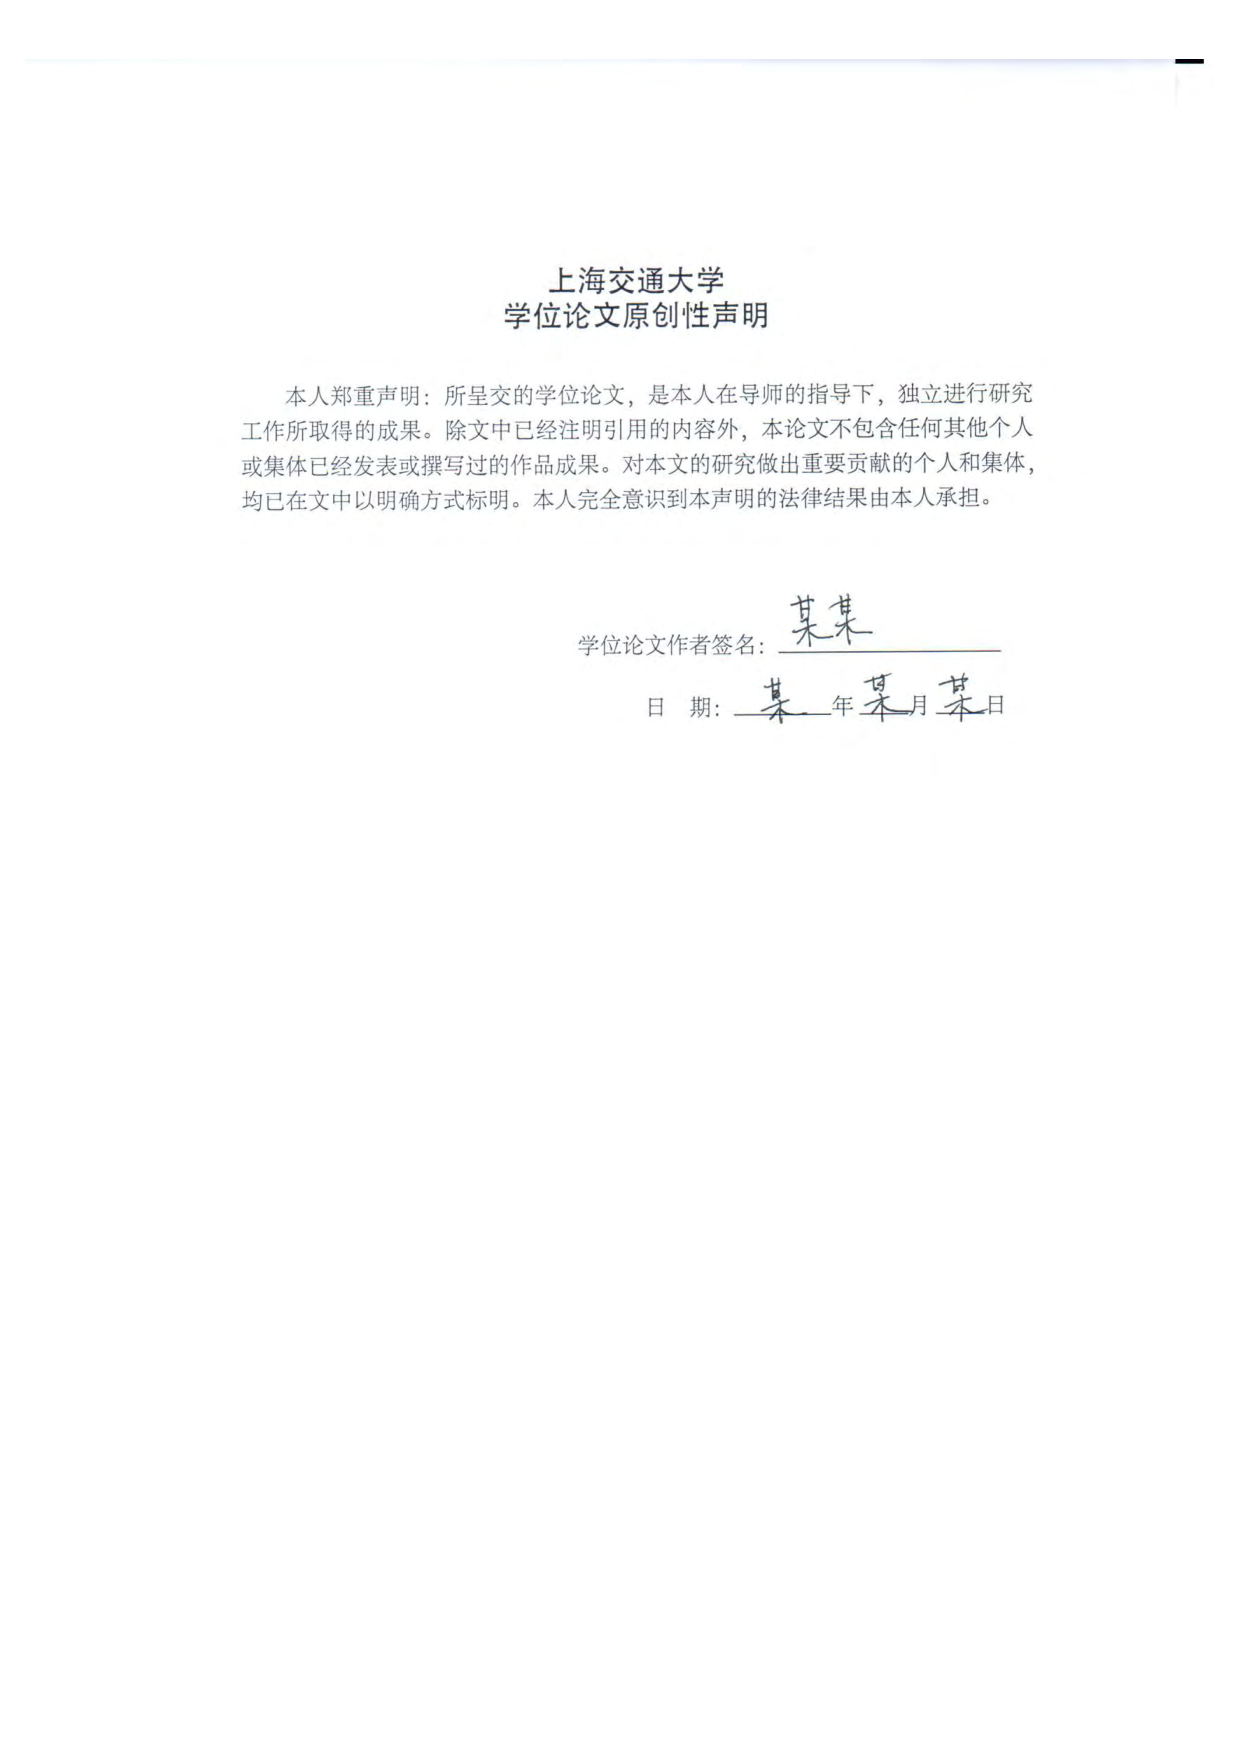
\includepdf{pdf/originality.pdf}
  \pdfbookmark[0]{\sjtu@label@originality}{originality}
  \cleardoublepage
  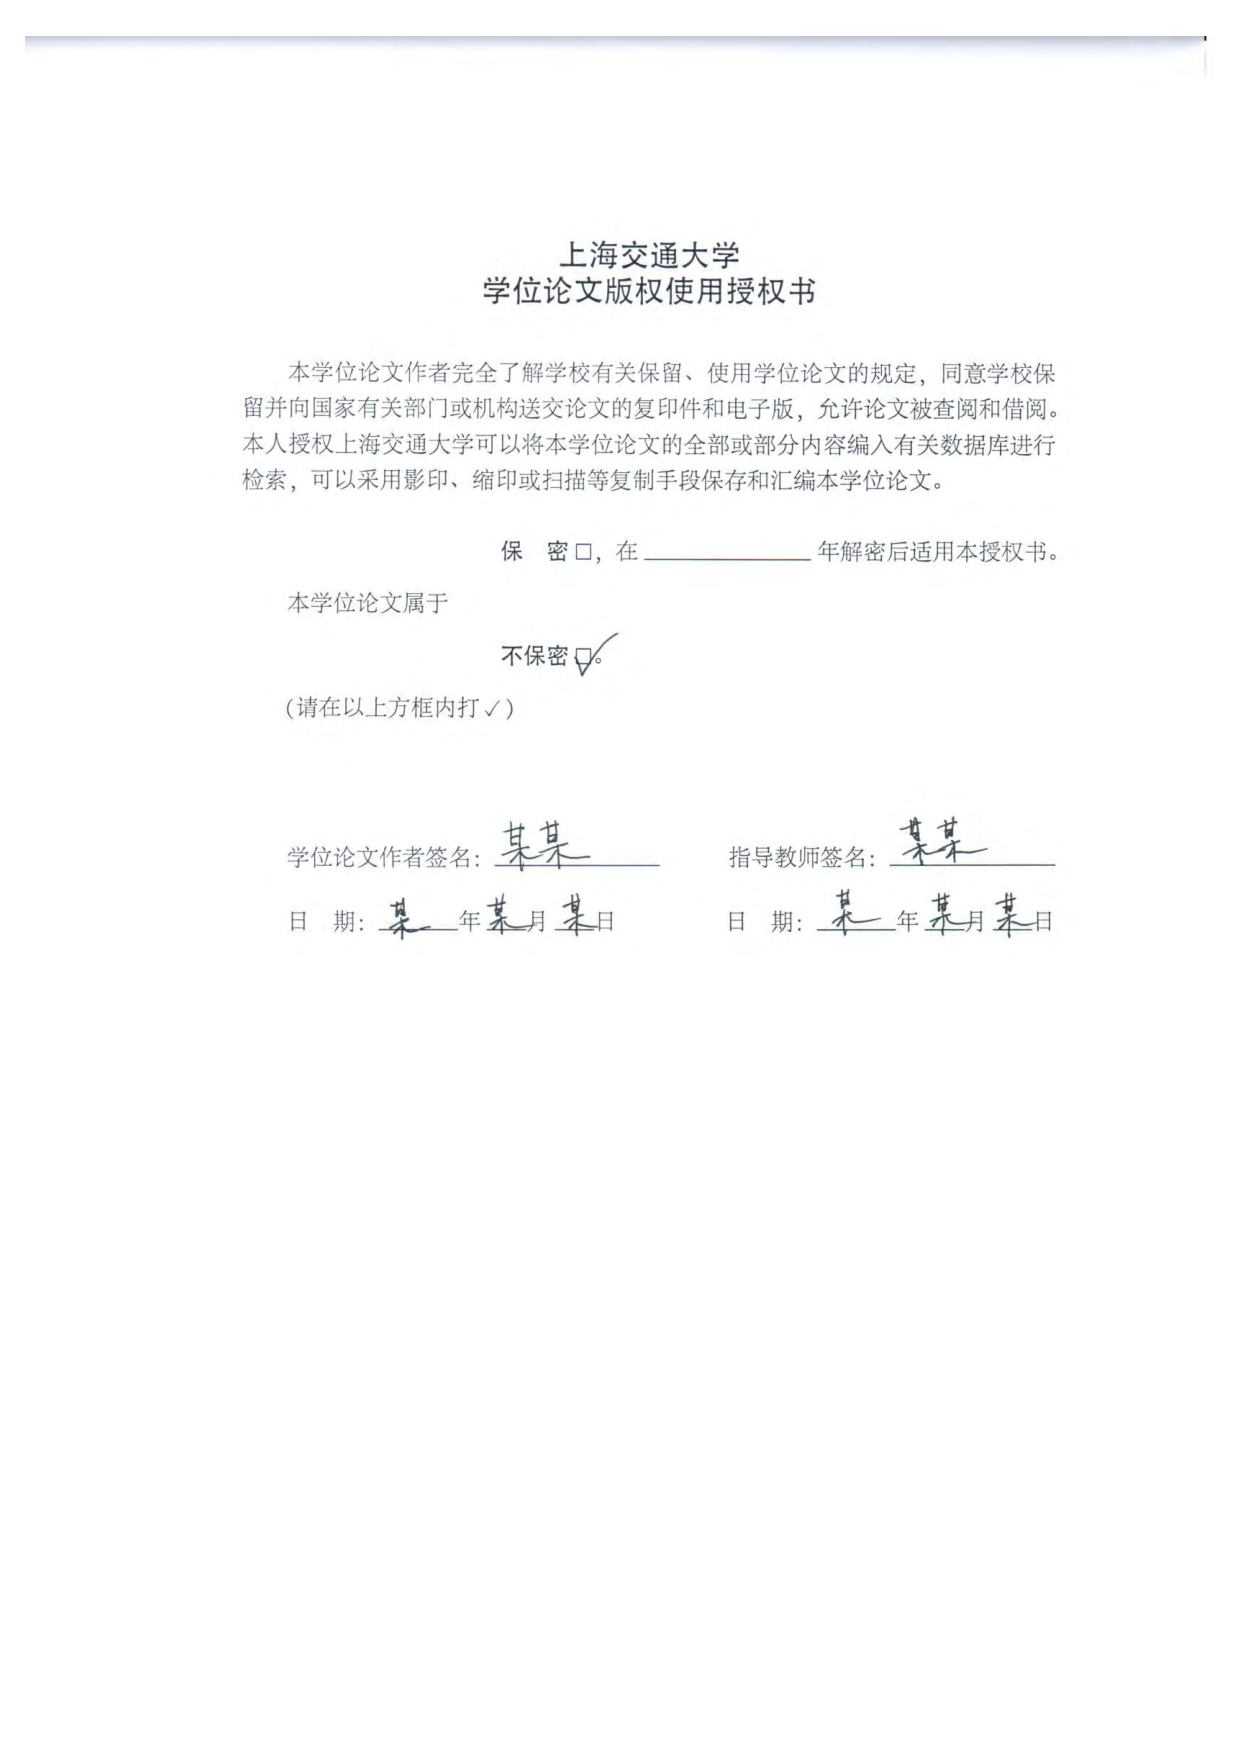
\includepdf{pdf/authorization.pdf}
  \pdfbookmark[0]{\sjtu@label@authorization}{authorization}
  \cleardoublepage
\else
\ifsjtu@review\relax
% exclude the originality and authorization declarations
\else
  \makeDeclareOriginality
  \makeDeclareAuthorization
\fi
\fi
\makeatother

%---------------------------------------------------------------------
\frontmatter

%%
%% Copyright (c) 2018 Weitian LI <liweitianux@sjtu.edu.cn>
%% Creative Commons BY 4.0
%%

% 中文摘要,约 3000 字
\begin{abstract}
\acl*{rh}如何影响 EoR 探测...
\end{abstract}

%---------------------------------------------------------------------

\begin{englishabstract}
\acs*{rh} can impose serious contamination on the EoR detection ...
\end{englishabstract}


\tableofcontents
\listoffigures
\addcontentsline{toc}{chapter}{\listfigurename}
\listoftables
\addcontentsline{toc}{chapter}{\listtablename}
% \listofalgorithms
% \addcontentsline{toc}{chapter}{\listalgorithmname}

\printacronyms[
  include-classes=symbol,
  name={主要符号对照表},
]

%---------------------------------------------------------------------
\mainmatter
\pagestyle{main}

%%
%% Copyright (c) 2018-2019 Weitian LI <liweitianux@sjtu.edu.cn>
%% Creative Commons BY 4.0
%%

\chapter{绪论}
\label{chap:introduction}

%=====================================================================
\section{研究背景}
\label{sec:background}

理解宇宙的结构、起源和演化,是人类孜孜不倦地追求的目标,在哲学和科学中占据重要地位.
经过无数人的努力,宇宙学的\ac{bbt}终于得以建立.
该理论已被大量观测证据所支持,比如星系的红移--距离关系(即 Hubble 定律)、
\ac{cmb}辐射、星系的大尺度分布、早期元素丰度、等等,
是目前宇宙学的标准模型.

根据大爆炸宇宙学模型,宇宙起源于约 138 亿年前的一次大爆炸,然后随着宇宙的膨胀,
温度以及能量密度都逐渐降低,宇宙主要经历了\ac{inflation}、\ac{bbn}、
\ac{recomb}、\ac{da}、形成第一代天体、\ac{reion}、形成星系及大尺度结构
等阶段,如\autoref{fig:univ-history} 所示.

\begin{figure}[!htp]
  \centering
  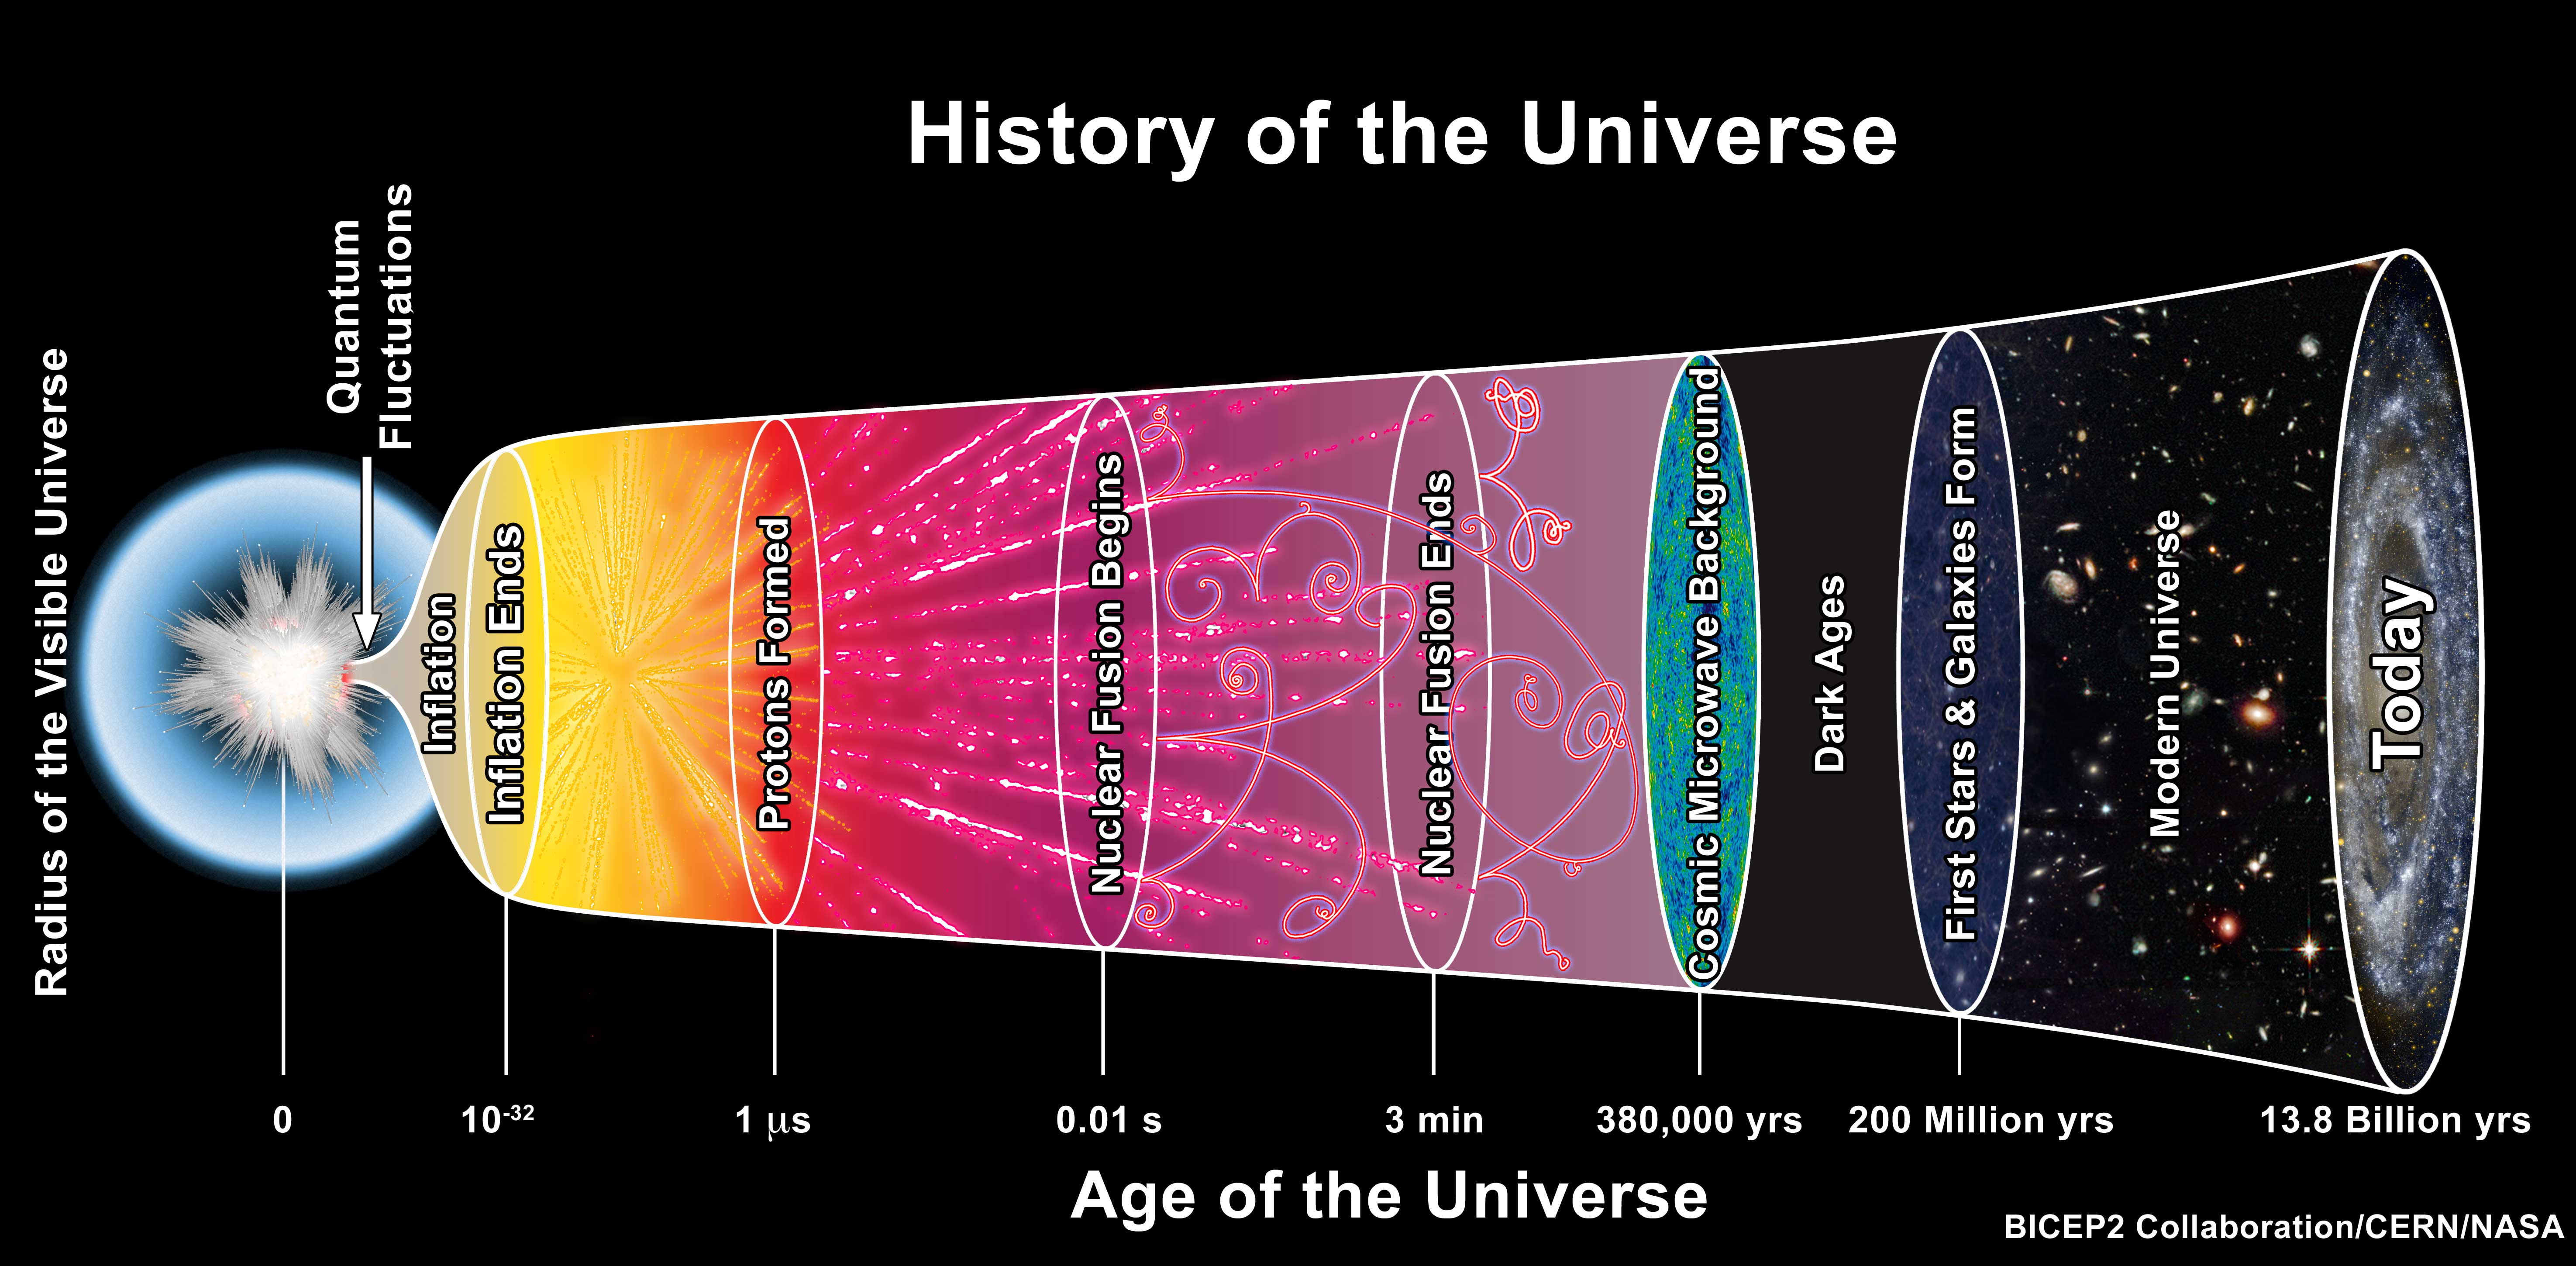
\includegraphics[width=\textwidth]{universe-history}
  \bicaption[宇宙的演化历史]{%
    宇宙从大爆炸到今天的演化历史.
  }{%
    The evolution of the Universe from the Big Bang
    to the present.
    \\\textcopyright{}
    \acuse{bicep,cern,nasa}
    \acs{bicep}2/\acs{cern}/\acs{nasa}; CC0 1.0.
  }
  \label{fig:univ-history}
\end{figure}

大爆炸之后约 40 万年,宇宙已冷却至大约 \SI{3000}{\kelvin},
于是自由电子被结合到中性原子之中,与重子物质脱耦的光子开始在宇宙中自由传播,
形成弥漫于整个宇宙的背景辐射,即今天所探测到的 \ac{cmb} 辐射.
但是,此时尚未形成发光的天体,因此宇宙进入了\acl{da}.
随着物质的密度扰动在引力作用下增长,第一代天体开始形成并产生辐射,使得重子物质
再次被逐步电离,宇宙从此结束\acl{da}并走入\ac{eor}.
随着各尺度上的天体结构的逐步形成与演化,重子物质被充分电离,宇宙也演化形成今天的格局.

\begin{figure}[!htp]
  \centering
  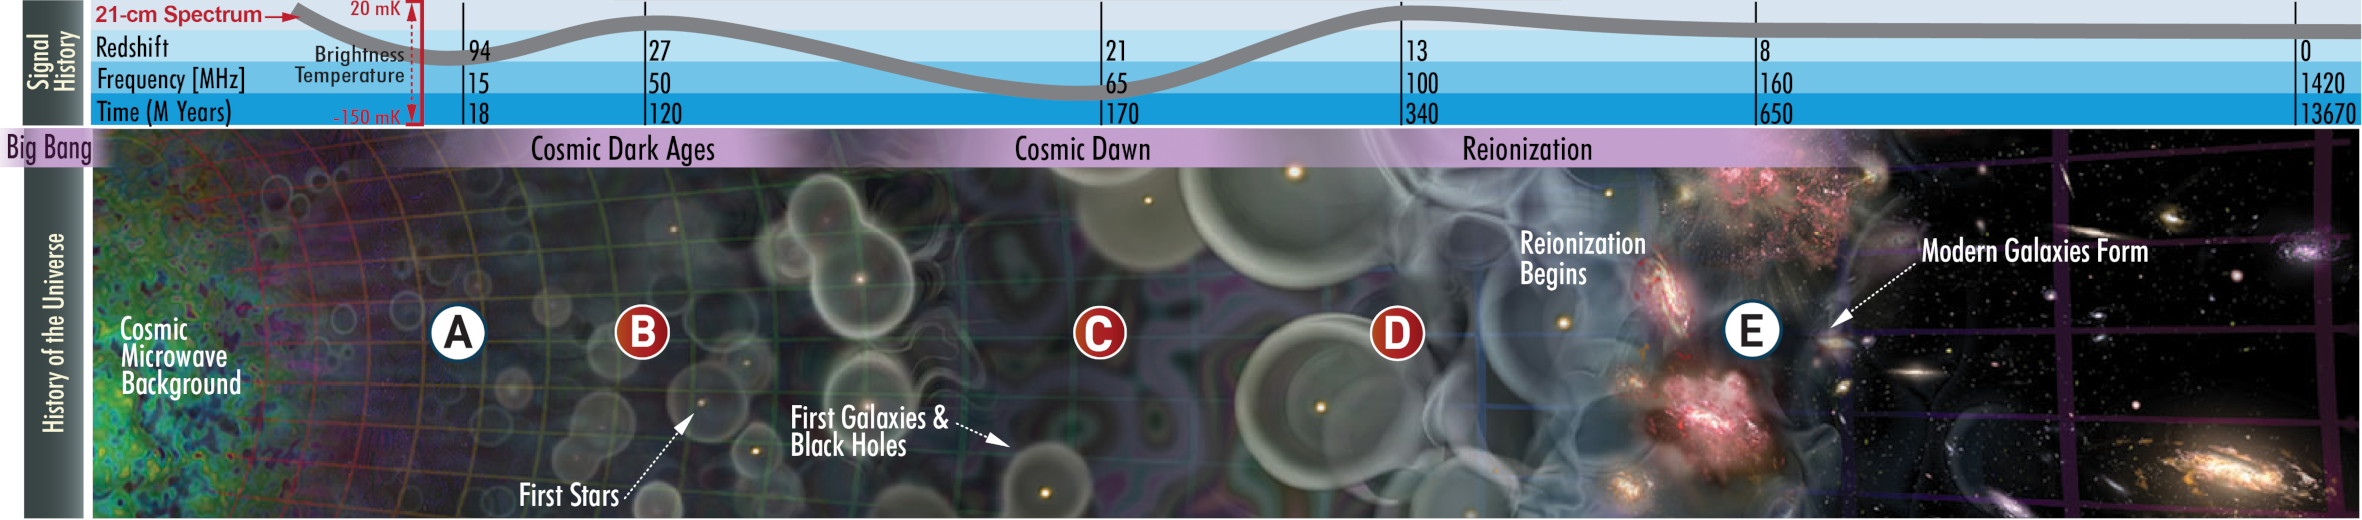
\includegraphics[width=\textwidth]{cosmic-stages-dare}
  \bicaption[宇宙的黑暗时期与再电离时期示意图]{%
    宇宙的\acl{da}与\acl{eor}示意图,其中显示了\acl{aoi} (A)、\acl{da} (B)、
    \acl{cd} (C) 以及\acl{eor} (D, E).
    上方的粗曲线显示了理论预测的 \hisignal/的强度.
  }{%
    A schematic showing the \acs{da} and the \acs{eor}
    of the Universe, mainly including the \acs{aoi} (A),
    the \acs{da} (B), the \acs{cd} (C), and the \acs{eor} (D, E).
    The thick curve in the top panel shows the predicted intensity
    of the 21\,cm signal.
    \\\textcopyright{}
    \acuse{dare}\ac{dare},
    \url{http://lunar.colorado.edu/dare/science.html}, (2018-09-23).
  }
  \label{fig:cosmic-stages}
\end{figure}

我们已借助多波段观测掌握了大量有关宇宙近期演化
($\acs{z} \lesssim 6$;宇宙已充分电离之后)的信息;
通过研究 \ac{cmb},我们对宇宙的早期历史
($z \gtrsim 1100$;自由电子\acl{recomb}之前)有了深刻理解.
然而,我们对中间的那段时期($z \sim \numrange{6}{1100}$)却知之甚少.
这段时期可细分为以下四个阶段\cite{koopmans2015}:
\acl{aoi} (\acs{aoi}; $z \sim \numrange{200}{1100}$)、
\acl{da} ($z \sim \numrange{30}{200}$)、
\acl{cd} (\acs{cd}; $z \sim \numrange{15}{30}$)
以及\acl{eor} ($z \sim \numrange{6}{15}$),
如\autoref{fig:cosmic-stages} 所示.
对于其中距离我们相对较近的\acl{eor},
我们目前仅获得非常有限的间接观测信息,比如:
该时期的\ac{hi}对高红移类星体的 Ly$\alpha$ 吸收 \cite{becker2001}、
该时期的自由电子对 \ac{cmb} 光子的 Thomson 散射 \cite{kaplinghat2003}.
但是,我们仍然缺乏来自\acl{eor}的直接观测证据,
对该时期的基本性质和关键物理过程仍不清楚,比如:
第一代天体是何时以及如何形成的?
主要的电离源有哪些以及它们是如何影响再电离过程的?
电离氢区的尺度以及演化过程如何?
研究\acl{eor}的对于理解宇宙早期结构形成以及星系的形成与演化有重要意义,
是建立完整的宇宙演化图景的关键环节之一.
具体请参见 \citeay{fan2006}, \citeay{morales2010},
\citeay{pritchard2012}, \citeay{zaroubi2013},
\citeay{koopmans2015} 等综述文.

在\acl{eor}及其之前的\acl{da},尽管缺乏发光天体可供观测,
但是宇宙中丰富的\acl{hi}所辐射的 21\,cm 谱线
(以下简称 \emph{\hisignal/};
详见 \autoref{sec:21cm-signal})为探测该时期提供了有效途径.
对 \hisignal/的探测是目前对\acl{eor}及其之前的\acl{da}开展系统性
研究的最直接而有效的观测手段 \cite{koopmans2015,furlanetto2016}.

\acl{hi}的 21\,cm 谱线的本征频率约为 \SI{1420}{\MHz}.
源自\acl{eor}的 \hisignal/(以下简称 \emph{EoR 信号})经历显著红移后
应出现在约 \SIrange{90}{200}{\MHz},对应低频射电波段.
EoR 信号到达地球时已非常微弱,仅约几 \si{\mK} 至十几 \si{\mK},
因此需要具有极高灵敏度的低频观测设备才能捕获该信号.
目前的主流技术是采用大规模低频干涉阵列,已建成或正在建设的干涉阵列主要有:
\ac{21cma} \cite{zheng2016}、
\ac{gmrt} \cite{paciga2011}、
\ac{mwa} \cite{bowman2013,tingay2013}、
\ac{lofar} \cite{vanHaarlem2013}、
\ac{lwa} \cite{ellingson2009}、
\ac{paper} \cite{parsons2010}、
\ac{hera} \cite{deboer2017}、
\ac{ska} \cite{mellema2013,koopmans2015}.
然而,利用干涉阵列探测 EoR 信号仍面临诸多困难与挑战,其中主要包括:
识别并扣除强烈的前景干扰、扣除人工源的\ac{rfi}、修正电离层的扰动、
苛刻的仪器校准要求、海量数据处理和高动态范围成像.

在低频射电波段,强烈的前景干扰(主要源自银河系以及河外点源;
详见 \autoref{sec:fg-intro})比待探测的 EoR 信号高出约 5 个数量级;
即便按干涉阵列所测量的天空亮度涨落来衡量,前景干扰的涨落也是待测信号的数千倍
\cite{zaroubi2013}.
如何准确把握前景干扰并将其有效扣除,是成功探测 EoR 信号的关键.
由于低频射电观测和巡天数据的严重不足,我们对该波段的前景的了解非常有限,
无法达到探测 EoR 信号所要求的精度.
因此,我们需要挖掘已有海量的中高频射电观测以及其他多波段观测数据,
并结合逐渐增长的低频观测数据,深入理解低频射电前景辐射,构建并完善前景模型,
为识别并扣除前景干扰提供有力支撑.

虽然在本质上,前景辐射的频谱是光滑的,而 EoR 信号的频谱呈锯齿状,
两者具有很好的可区分性 \cite{wang2006,jelic2008,harker2009,wang2013}.
然而在实际情况中,受到干涉阵列的复杂仪器效应、观测干扰、数据处理技术的限制
等因素的影响,前景频谱的光滑性遭到破坏,导致 EoR 信号的提取变得尤其困难
\cite{liu2009ps,labropoulos2009,gehlot2018,mertens2018}.
如何研发出行之有效的前景处理和 EoR 信号提取算法,亦是当前的重要研究课题.


%=====================================================================
\section{研究内容}
\label{sec:content}

本文的研究内容分为以下两部分:
\begin{itemize}
\item
\emph{改进低频射电天空的模拟:}
深刻理解各前景成分的性质(如强度、空间分布、频谱结构)并充分把握它们对 EoR 探测
的干扰方式,是研发具有针对性的前景去除和 EoR 信号分离算法的前提与关键 (ref???).
由于复杂的仪器效应和严重的观测干扰,低频干涉阵列的系统校准非常困难
\cite{noordam2004,intema2009,wijnholds2010,barry2016,gehlot2018},
严重制约仪器达到探测 EoR 信号所要求的极高灵敏度.
在现阶段缺乏足够可用的高质量低频射电观测数据的情况下,挖掘已有多波段观测数据并
准确模拟低频射电天空,是开展前景干扰研究以及 EoR 信号分离算法研发的可行办法.

\hspace{2\ccwd}%
在诸多前景成分之中,银河系的弥散辐射 [包括\ac{synrad}和\ac{brad}]
以及河外\ac{pntsrc}辐射是最主要的成分,目前已被广泛地研究和较好地理解
\cite{shaver1999,diMatteo2004,gleser2008,liu2012,murray2017,spinelli2018}.
除此之外,剩下的前景辐射主要来自河外\ac{extsrc},其中包括:
\ac{icm} \cite{feretti2012} 产生的\ac{rh}、\ac{rr}和\ac{rmh}、
\ac{gc}之外的\ac{igm} \cite{keshet2004}、
以及\ac{lsf} \cite{vazza2015}.
对于这些河外\acl{extsrc},已获得的观测证据不多,在低频射电波段更是不足.
关于它们将具体如何影响 EoR 探测,目前的理解非常有限,亟待深入且系统的研究.

\hspace{2\ccwd}%
与其他几类河外\acl{extsrc}相比,\acl{rh}拥有更多的观测证据和理论研究,支撑我们
构建一个更佳的模型用来模拟\acl{rh}的低频射电辐射,改进低频射电天空的模拟,
进而在考虑干涉阵列的实际仪器效应的情况下,有效地评估\acl{rh}对 EoR 探测的影响.

\item
\emph{研发 EoR 信号分离新算法:}
为了提取淹没于前景干扰中的 EoR 信号,一系列方法已被提出来用于处理前景
(详见 \autoref{sec:fg-methods}).
这些前景处理方法可大致分为\ac{fgrm}和\ac{fgavd}两大类,
但都依赖于一个重要前提:前景辐射的频谱必须非常光滑.
据此,这些方法通过构建一个模型来拟合光滑的前景成分并扣除,或者在功率谱空间尽量
避开前景污染区域,从而提取出微弱的 EoR 信号 \cite{chapman2016}.

\hspace{2\ccwd}%
然而在实际情况中,干涉阵列的\ac{beam}存在频率依赖效应(以下简称\emph{波束效应}),
即\acl{beam}的形状随观测频率而变化,因此 CLEAN 后残留的前景源会产生沿频率方向
快速变化的涨落,严重破坏前景频谱的光滑性 \cite{liu2009ps},
导致现有方法无法有效分辨前景干扰与 EoR 信号并分离出 EoR 信号
(详见 \autoref{sec:fdeffect}).

\hspace{2\ccwd}%
考虑到干涉列阵的\acl{beam}的形状非常复杂,为现有方法打造一个实际可用的模型
用以克服上述复杂的波束效应将很困难 \cite{lochner2015},
因此研发基于\ac{dl}的 EoR 信号分离新算法是一条更加可行且具有吸引力的途径
\cite{herbel2018,vafaeiSadr2019},
通过从数据中学习知识并自适应地优化模型,达到克服波束效应并分离 EoR 信号的目标.

\end{itemize}

本文的研究目标是:
(1)改进\acl{rh}的模拟,考虑干涉阵列的实际仪器效应,
获得更精细、更符合实际的低频射电天空的模拟图像,
进而有效地评估\acl{rh}对 EoR 探测的影响.
(2)研发基于\acl{dl}的能够有效克服干涉阵列的波束效应的 EoR 信号分离新算法,
并运用到上述模拟数据进行测试和优化.


%=====================================================================
\section{研究方案}
\label{sec:plan}

本文遵循以下主要步骤开展开展工作,完成研究内容,达到研究目标:
\begin{enumerate}
\item
调研\acl{rh}的相关理论研究和观测证据,理解其形成机制和演化规律,
构建模型并编程实现模拟\acl{rh}的低频射电辐射.
搜集\acl{rh}的现有观测数据,调节模型的参数,获得可靠的模拟结果.

\item
采用典型的干涉阵列(如 SKA1-Low)的布局方案,对上一步所得的\ac{skymap}
开展模拟观测,得到\ac{vis}数据,再利用 CLEAN 算法成像获得相应的“观测”图像.
通过这种\ac{e2e}模拟,干涉阵列的复杂仪器效应(如本文关注的波束效应)得以
有效地整合到研究流程之中.

\item
基于上述模拟所得的“观测”图像,利用一维和二维\ac{ps},对比\acl{rh}和
EoR 信号的异同,量化\acl{rh}在运用\acl{fgrm}或\acl{fgavd}的情况下
对 EoR 探测的影响,有效评估\acl{rh}作为前景干扰成分的重要程度.

\item
对比分析目前的主流\acl{dl}方法,筛选出合适的算法并加以必要的改进,
适用到此处的 EoR 信号分离场景.
利用已有模拟数据对算法进行训练和调优,挑选出满足要求的最佳算法.

\end{enumerate}


%=====================================================================
\section{本文框架}
\label{sec:structure}

本文余下章节安排如下:
\autoref{chap:interferometry}将介绍射电天文学和射电干涉技术的基础知识,
包括基本辐射理论、天线原理、干涉阵列及综合孔径成像等.
在\autoref{chap:detection},我们将介绍利用\acl{hi}
\hisignal/探测宇宙再电离时期的方法和困难、以及前景处理方法.
在\autoref{chap:simulation},我们首先模拟各前景成分和 EoR 信号的\acl{skymap},
然后进行干涉阵列的模拟观测,得到整合了实际仪器效应的观测图像.
据此,我们在\autoref{chap:halo}借助\acl{ps}量化评估\acl{rh}对
EoR 探测的具体影响.
\autoref{chap:cdae}将阐述我们提出的基于\acl{dl}的 EoR 分离新算法并演示其效果.
最后,我们对全文进行总结并简要展望.

全文采用一个由 \lcdm/ 模型描述的平直宇宙,具体参数为:
$\acs{H0} = 100\,\acs{h} = \SI{71}{\km\per\second\per\Mpc}$、
$\acs{Om0} = 0.27$、
$\acs{Ol0} = 1 - \acs{Om0} = 0.73$、
$\acs{Ob0} = 0.046$、
$\acs{ns} = 0.96$ 以及 $\acs{sigma8} = 0.81$.
如无额外说明,本文给出的误差对应 \SI{68}{\percent} 的置信水平;
使用的幂律谱形式为 $\acs{Sfreq} \propto \acs{freq}^{-\acs{Sidx}}$,
其中 \acs{Sfreq} 为\acl{Sfreq}、\acs{Sidx} 为\acl{Sidx}.
本文使用的中文术语遵循《英汉天文学名词数据库》
\footnote{英汉天文学名词数据库:\url{http://astrodict.china-vo.org/}}.


%% EOF

%%
%% Copyright (c) 2018 Weitian LI <liweitianux@sjtu.edu.cn>
%% Creative Commons BY 4.0
%%

\chapter{射电干涉技术基础}
\label{chap:interferometry}

%=====================================================================
\section{射电天文学简介}
\label{sec:radio-astronomy}

TODO

%---------------------------------------------------------------------
\subsection{射电天文学是什么?}

TODO

%---------------------------------------------------------------------
\subsection{射电窗口}

TODO

%---------------------------------------------------------------------
\subsection{机遇和挑战}

TODO


%=====================================================================
\section{辐射理论}
\label{sec:radiation}

TODO ...
spectral brightness $I_{\nu}$

%---------------------------------------------------------------------
\subsection{亮度和流量密度}

In the radio frequency regime, the Rayleigh-Jeans approximation
always holds, therefore the spectral brightness $I_{\nu}$ can be
equivalently expressed by \emph{brightness temperature} $T_b(\nu)$
through the relation \cite{condon2016}:
\begin{equation}
  \label{eq:Tb}
  T_b(\nu) \equiv \frac{I_{\nu} c^2}{2 k_B \nu^2}.
\end{equation}

%---------------------------------------------------------------------
\subsection{黑体辐射和亮温度}

TODO


%=====================================================================
\section{天线原理}
\label{sec:antenna}

TODO

%---------------------------------------------------------------------
\subsection{辐射方向图}

TODO

%---------------------------------------------------------------------
\subsection{增益和阻抗}

TODO

%---------------------------------------------------------------------
\subsection{主瓣和旁瓣}

TODO

ERA: eq:(3.96,3.118)

%---------------------------------------------------------------------
\subsection{有效面积}

TODO

%---------------------------------------------------------------------
\subsection{互易定理}

(???) TODO

%---------------------------------------------------------------------
\subsection{天线温度}

TODO


%=====================================================================
\section{干涉仪和综合孔径}
\label{sec:interferometer}

TODO

%---------------------------------------------------------------------
\subsection{基本原理}

TODO

二元干涉仪

%---------------------------------------------------------------------
\subsection{综合孔径}

TODO

坐标系统, 优点和缺点

%---------------------------------------------------------------------
\subsection{可视度}

TODO

%---------------------------------------------------------------------
\subsection{\texorpdfstring{$uv$}{uv} 覆盖}

TODO

integration time, earth rotation, phase tracking

%---------------------------------------------------------------------
\subsection{三个波束}

antenna beam, (??? primary beam), station beam, sythesized beam (PSF)

%---------------------------------------------------------------------
\subsection{三个中心}

phase center, pointing center, delay center

phase tracking, drift scan

%---------------------------------------------------------------------
\subsection{灵敏度}

point-source sensitivity, brightness sensitivity

ERA: 3.6.3.2:confusion

%---------------------------------------------------------------------
\subsection{数字波束合成}

multi-beam, phased array, 优点和缺点

%---------------------------------------------------------------------
\subsection{脏图}

weighting (natural, uniform, robust/Briggs)

%---------------------------------------------------------------------
\subsection{CLEAN 算法}

TODO

%---------------------------------------------------------------------
\subsection{大视场成像}

$w$-term, $w$-projection, $w$-stacking


%=====================================================================
\section{主要低频干涉阵列}
\label{sec:instruments}

大型低频干涉阵列是目前测量 EoR 信号的主要设备。
近十几年以及,国内外已建成一批各具特色的低频干涉阵列,
还有若干新型干涉阵列正在兴建或准备建设。
以下对其中主要的干涉阵列作简要介绍。

%---------------------------------------------------------------------
\subsection{21CMA}

\acf{21cma} 是我国开展“宇宙第一缕曙光”探测的低频射电干涉阵列,
位于中国西部天山深处的乌拉斯台,环绕在四周的高山能提供宁静的射电环境。
\acs{21cma} 的 81 个站点呈 T 形分布在东西约 \SI{6}{\km}、
南北约 \SI{4}{\km} 的两条直线上
(\autoref{fig:21cma} 展示了沿东西方向的部分站点)。
每个站点包含 127 根对数周期天线,工作频率为 \SIrange{50}{200}{\MHz},
频率分辨率为 \SI{24.4}{\kHz},
角分辨率达 \SI{1}{\arcminute}(在 \SI{200}{\MHz} 处),
采用模拟波束合成固定观测以北天极为中心、半径约 \SI{5}{\degree} 的天区
\cite{wang2013,zheng2016}。
\acs{21cma} 已于 2006 年建设完成,并于 2009 年升级了新型低噪声放大器和
基于 \acs{gpu} 的数据采集系统,目前已积累多年的观测数据。
\acs{21cma} 作为中国主要的 \acs{ska} 探路者项目,
项目成员开发了完整的数据处理流程及软件、
提出了射频干涉探测及抑制新方法 \cite{huang2016}、
探测并编录了北天极视场内的 624 个射电源 \cite{zheng2016}。
目前,\acs{21cma} 正在改造升级数字多波束合成系统,
以实现多目标跟踪观测,掌握低频脉冲星的搜寻技术。

\begin{figure}[!htb]
  \centering
  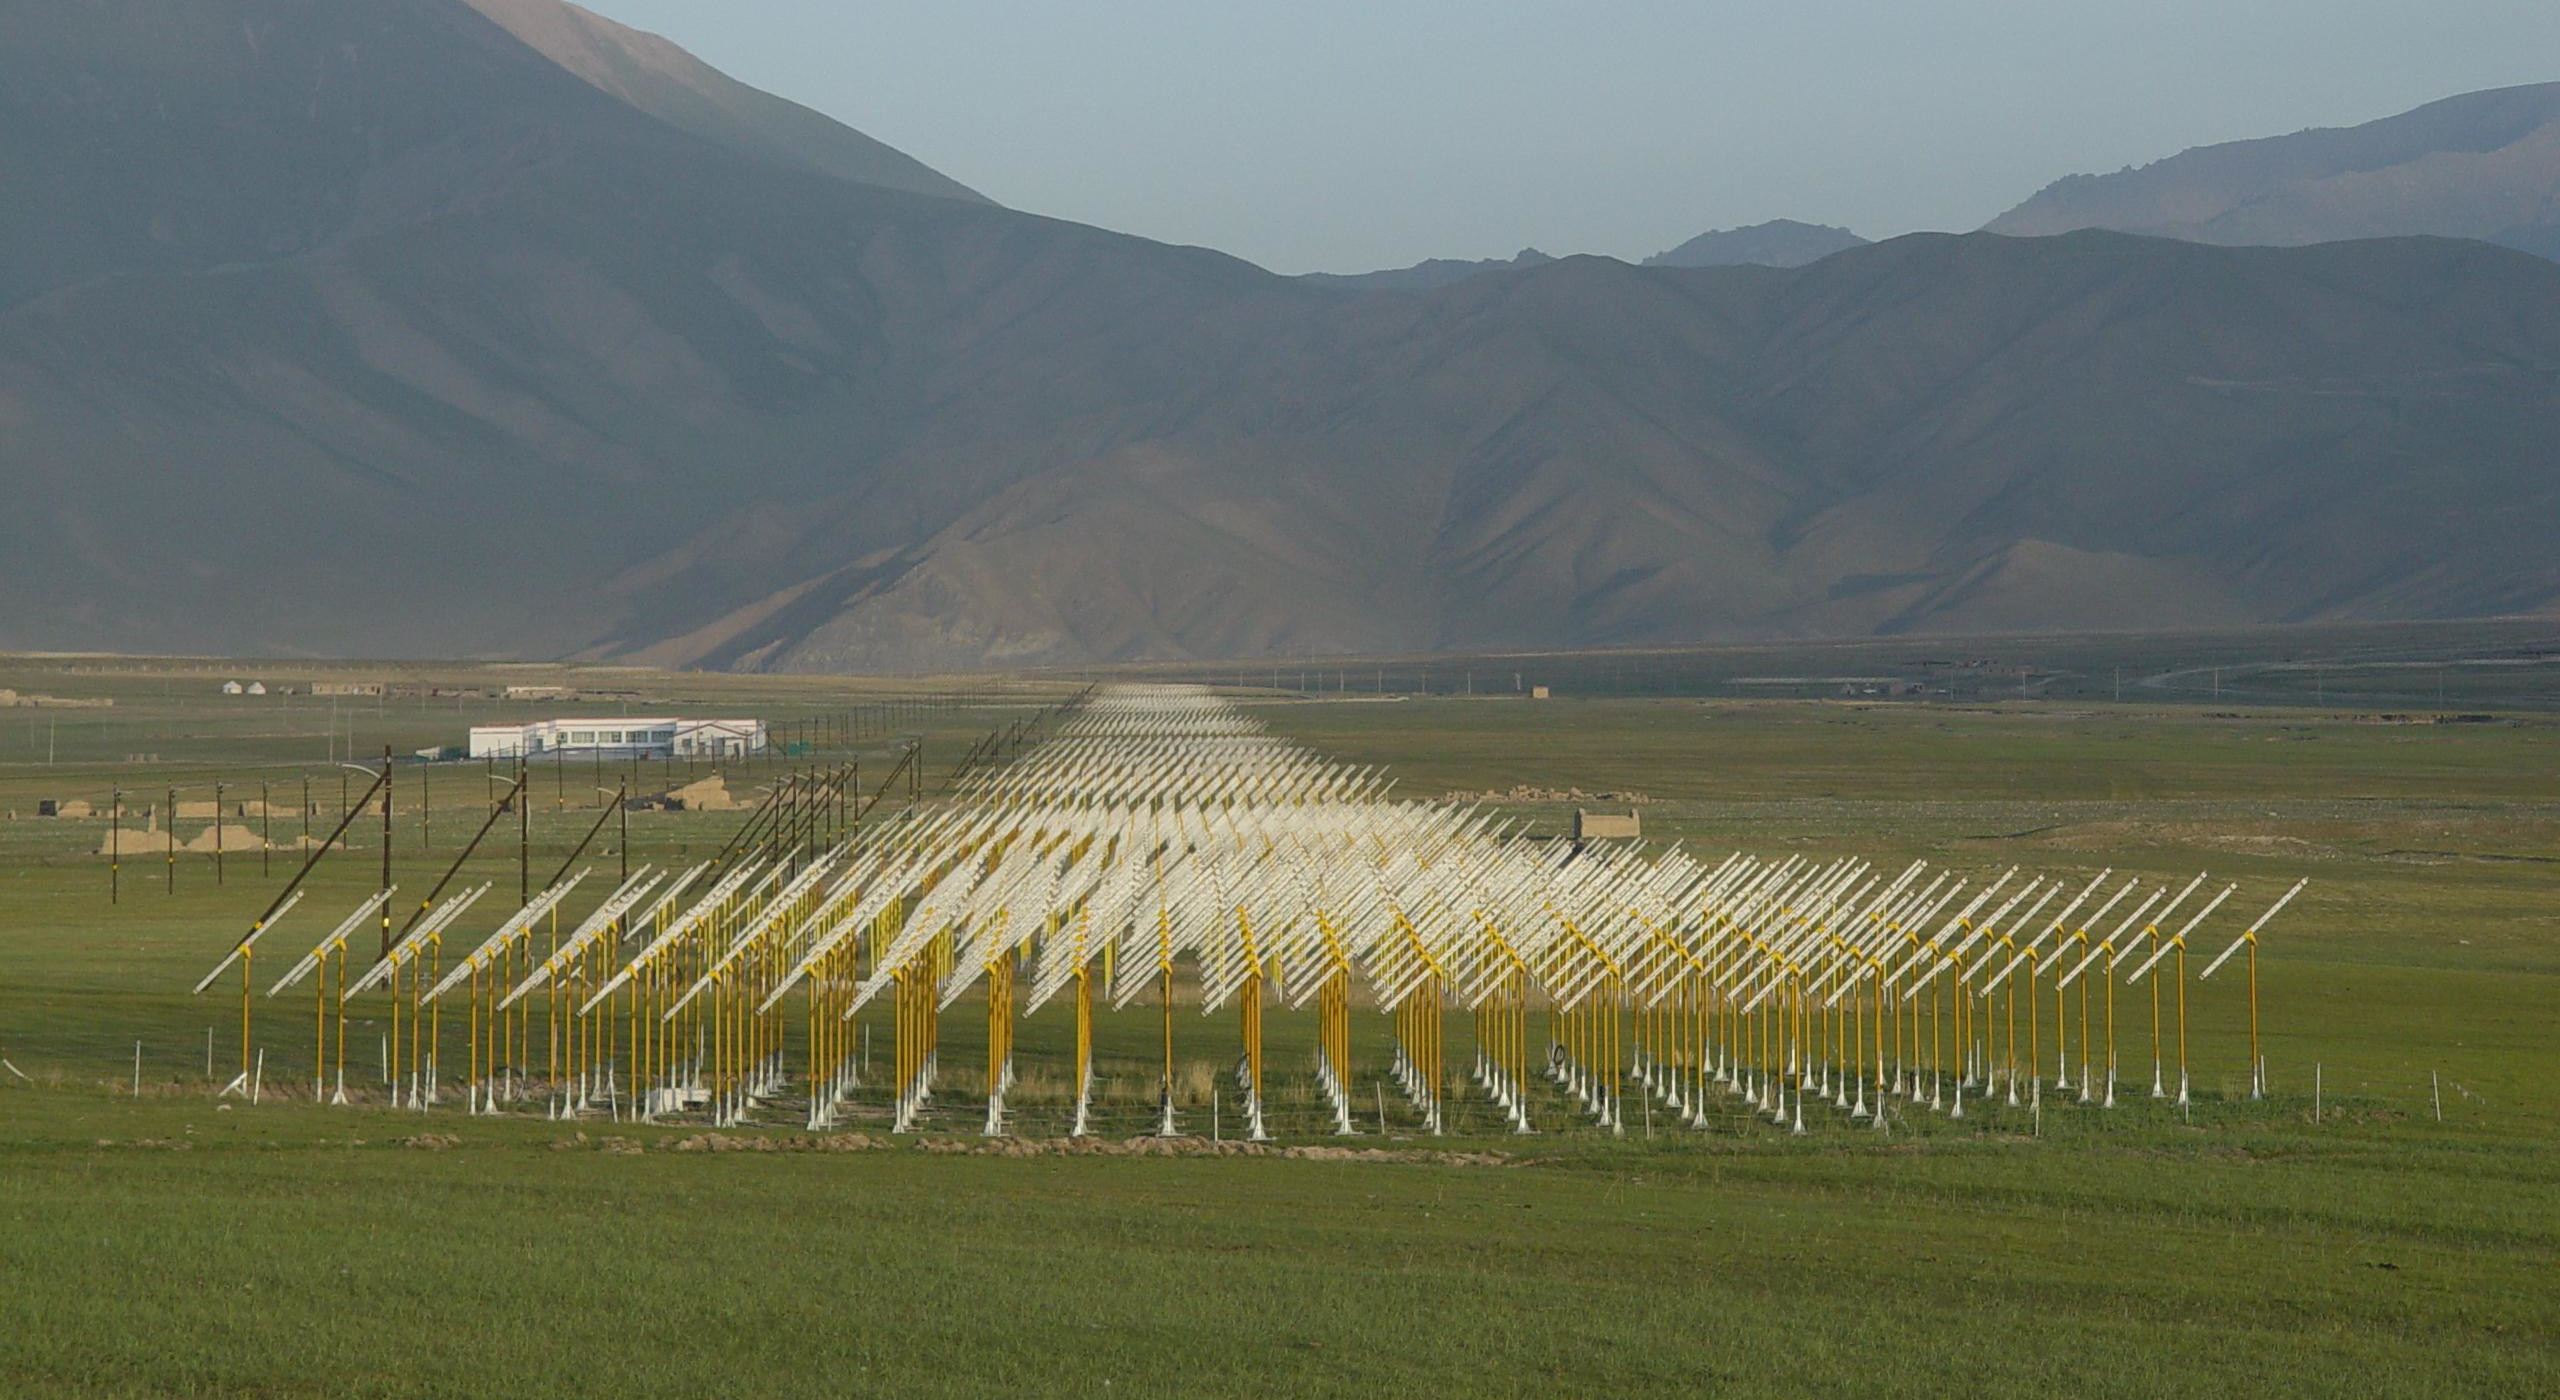
\includegraphics[width=0.8\textwidth]{21CMA}
  \bicaption[\acs{21cma} 东西方向的部分站点]{%
    \acs{21cma} 东西方向的部分站点,每个站点包含 127 根对数周期天线。
  }{%
    Part of the \acs{21cma} stations along the east-west direction,
    with each station including 127 log-periodic antennas.
    \\\textcopyright{}
    \acs{21cma}, \acl{nao}.
  }
  \label{fig:21cma}
\end{figure}

%---------------------------------------------------------------------
\subsection{LOFAR}

digital beamforming, multiple beams; SKA precursor ...

\acf{lofar} 是由\ac{astron}设计和建造的创新性的低频干涉阵列
\cite{vanHaarlem2013} (ref???),
由工作在 \SIrange{10}{90}{\MHz} 波段的低频段天线(LBA)和
工作在 \SIrange{110}{250}{\MHz} 波段的高频段天线(HBA)两部分组成。
\acs{lofar} 共有 51 个站点,
其中 24 个站点分布在半径 \SI{2}{\km} 的核心区域
(\autoref{fig:lofar} 显示了最中心的部分),
14 个站点呈螺旋状分布在外围区域,
还有 13 个国际站点分布在德国、法国、瑞士、英国、波兰和爱尔兰,
基线长达 \SI{1500}{\km}。
荷兰境内的 38 个站点各包含 96 个 LBA 和 48 个 HBA,
13 个国际站点每个包含 96 个 LBA 和 96 个 HBA。
\acs{lofar} 采用了数字多波束合成技术,能实现多目标跟踪观测,
并且显著提高巡天效率,为 \acs{ska1low} 提供强有力的技术支持
\cite{vanHaarlem2013} (ref???)。
\acs{lofar} 于 2012 年建设完成并开始观测,
已经完成北天 \SIrange{120}{168}{\MHz} 的深度巡天
\ac{lotss} \cite{shimwell2017}。
目前,\acs{lofar} 正在提议 2.0 升级计划 (ref???)。

\begin{figure}[!htb]
  \centering
  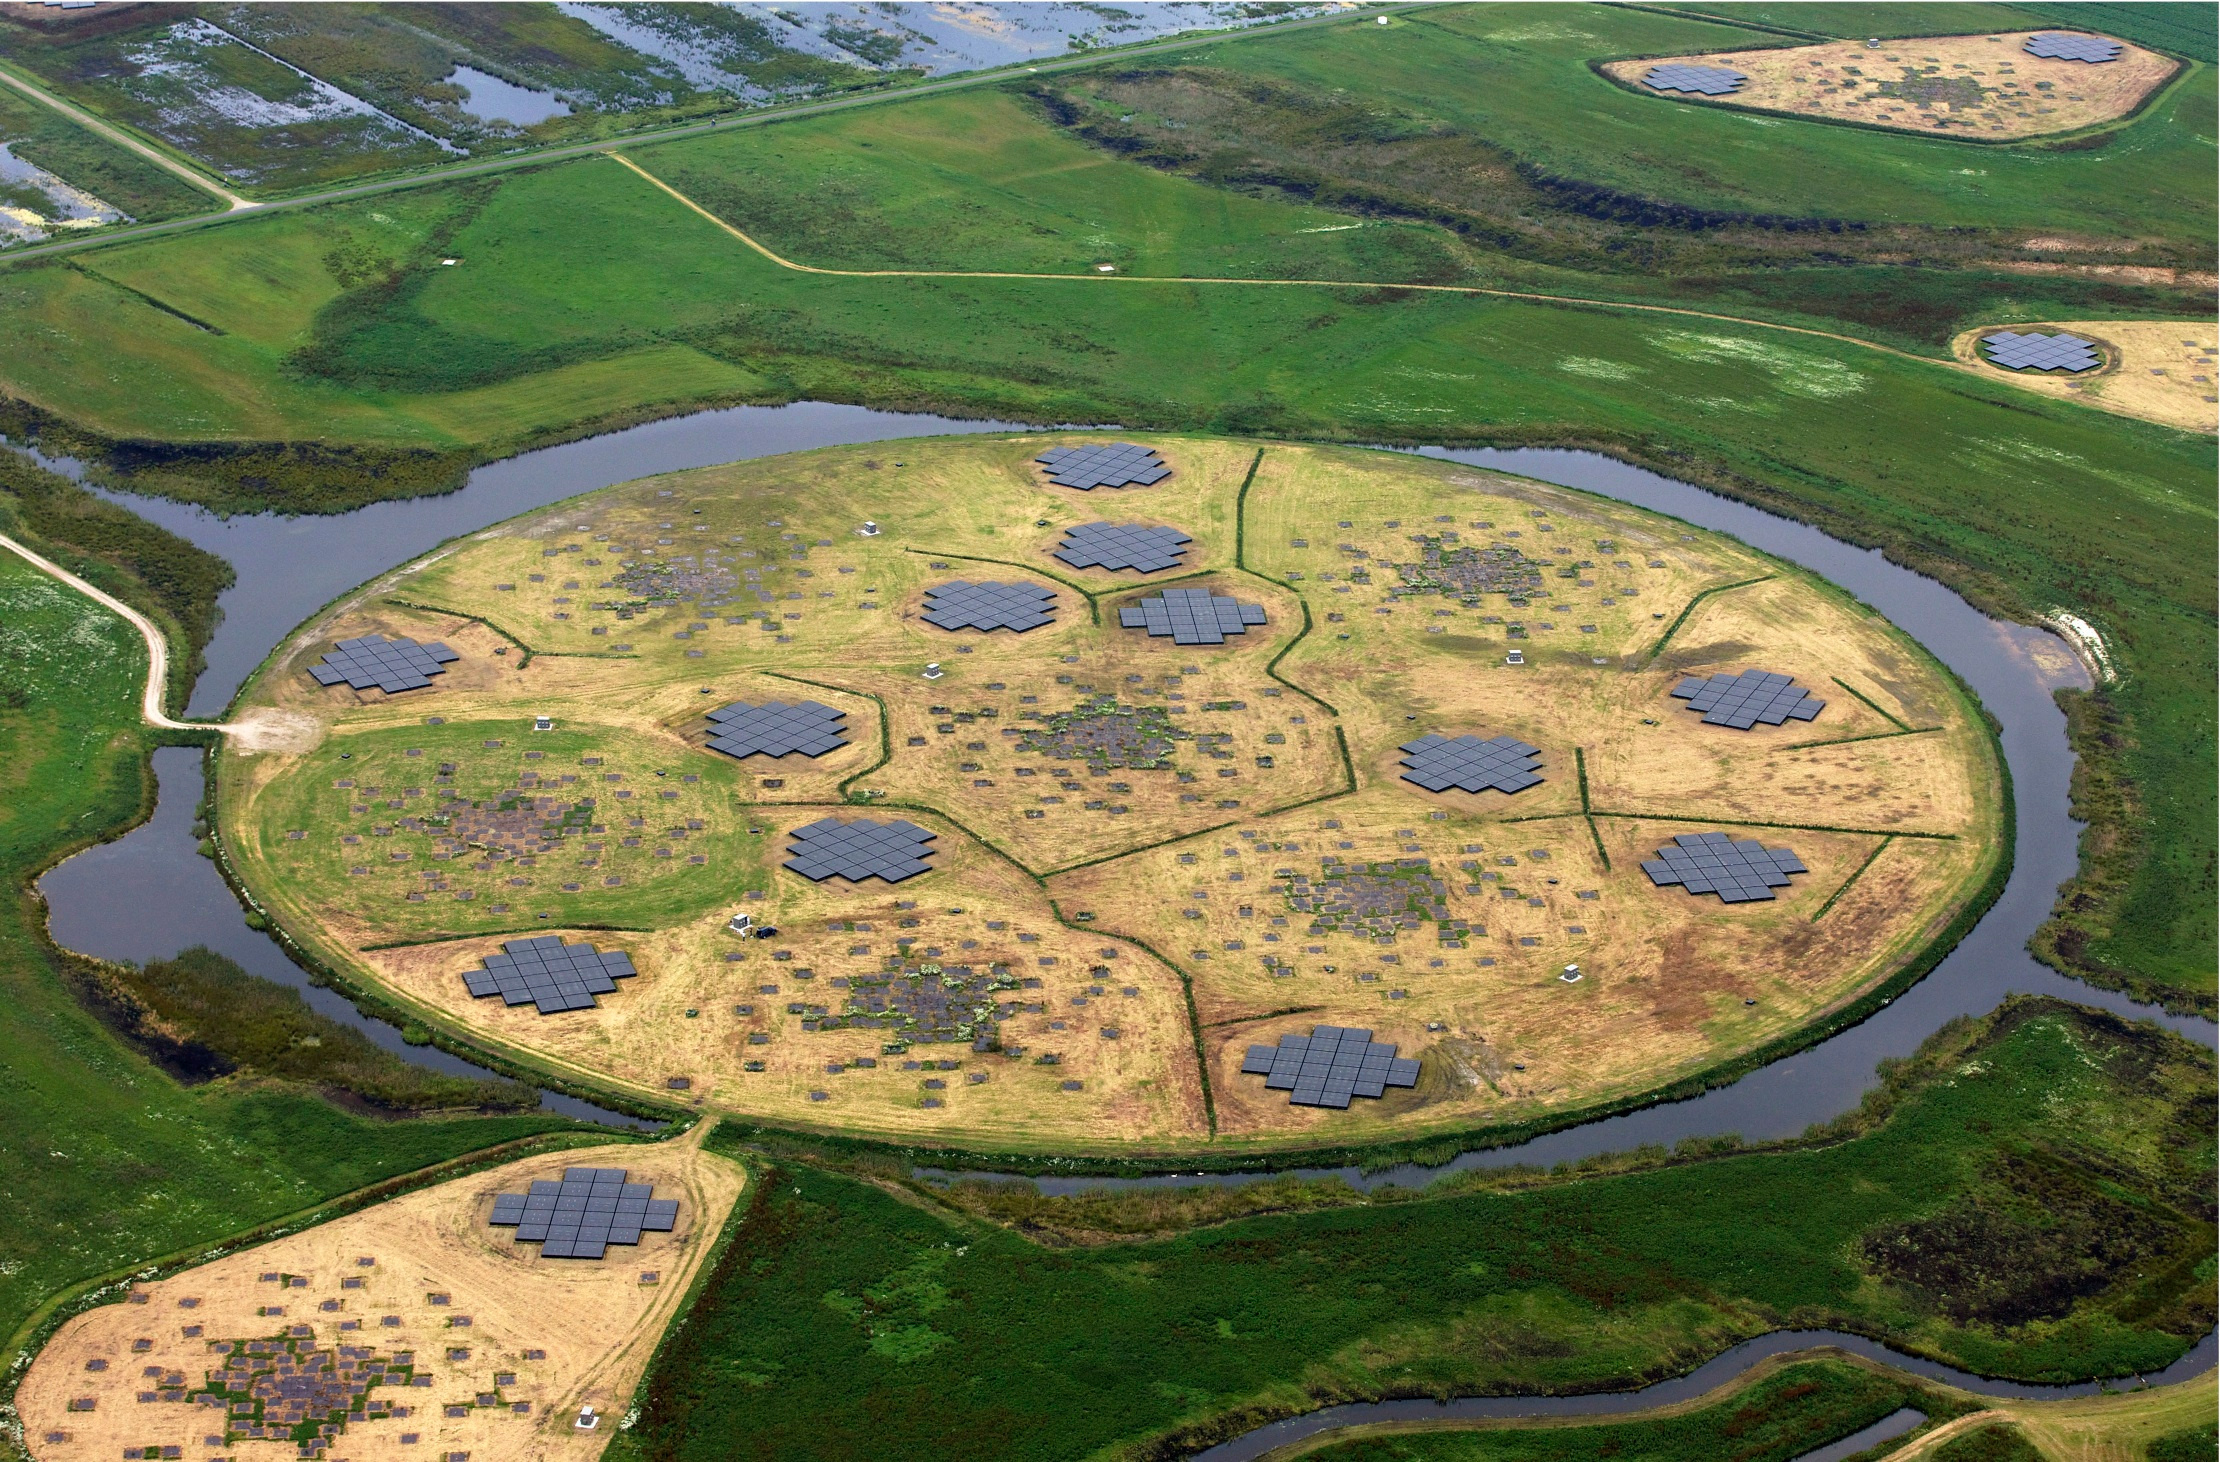
\includegraphics[width=0.8\textwidth]{LOFAR-superterp}
  \bicaption[\acs{lofar} 核心区域的中心]{%
    \acs{lofar} 核心区域的中心。
    小块深色区域为 LBA,大块深色区域为 HBA。
  }{%
    The heart of the \acs{lofar} core.
    The small dark regions are installed with LBA,
    while the big dark regions are installed with HBA.
    \\\textcopyright{}
    \textcite{vanHaarlem2013}.
  }
  \label{fig:lofar}
\end{figure}

%---------------------------------------------------------------------
\subsection{MWA}

compact + extended configurations; SKA precursor ...

\acf{mwa} 位于澳大利亚西部的 Murchison 射电天文台,
是 \acs{ska1low} 的探路者阵列 \cite{bowman2013,tingay2013}。
该阵列的主要科学目标包括宇宙再电离信号探测、河内及河外射电源、暂现源和空间天气研究。
\acs{mwa} 工作在 \SIrange{80}{300}{\MHz} 频段,使用一种双极化偶极子天线,
每个站点包含 16 个天线(按 4 行 4 列规则排列)。
所有天线均固定指向天顶,工作时通过调控各天线的时延来控制波束合成与指向。
\acs{mwa} 的特点为大视场和高表面亮度灵敏度 (???)。
\acs{mwa} 自 2007 年开始建设,于 2012 年完成了一期 128 个站点的建设,
于 2017 年底完成了二期 128 个新站点的扩建工作,目前已投入使用。
\autoref{fig:mwa} 显示了 \acs{mwa} 东侧六边形区域内的站点。
使用 \acs{mwa} 一期完成的 \ac{gleam} 巡天项目已发布一批成果,
包括点源目录 \cite{hurleyWalker2017}。。。
使用 \acs{mwa} 二期开展的 \ac{gleam-x} 巡天也正在积极进行 (ref???)。
作为少有的覆盖南天的低频射电巡天,\acs{gleam} 和 \acs{gleam-x}
将为 \acs{ska1low} 的巡天工作提供校准指导和星表的交叉认证。
同时 \acs{mwa} 也将会为 \acs{ska1low} 的宇宙再电离探测任务提供
更精准的天空模型和天区指导。

\begin{figure}[!ht]
  \centering
  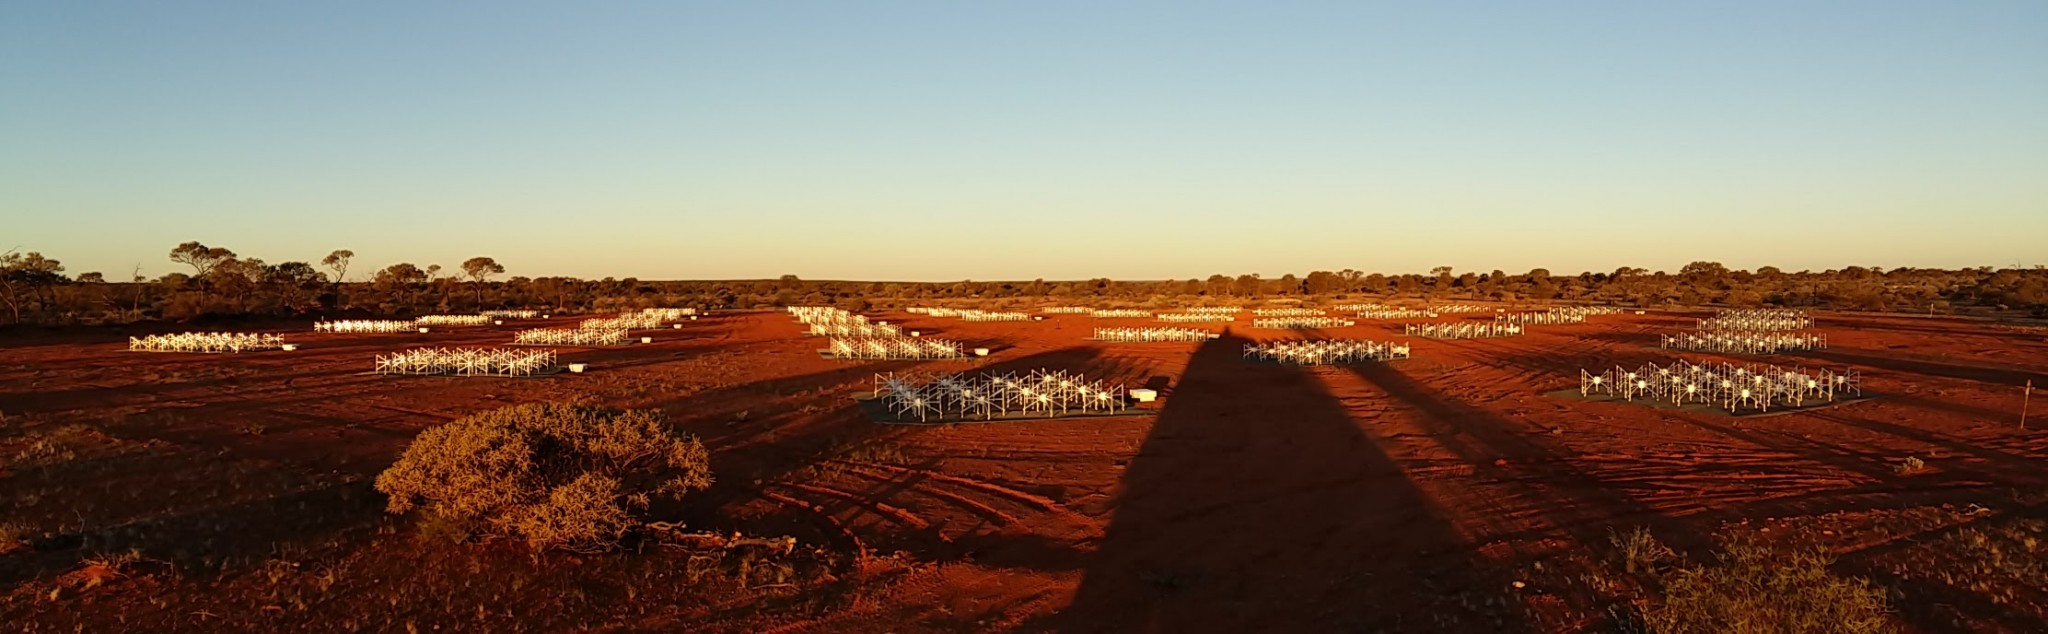
\includegraphics[width=\textwidth]{MWA}
  \bicaption[\acs{mwa} 东部站点]{%
    \acs{mwa} 东侧六边形区域内的站点,每个站点包含 16 个天线。
  }{%
    The stations inside the \acs{mwa}'s east hexagonal region,
    with each station consisting of 16 antennas.
    \\\textcopyright{}
    \acuse{icrar}\ac{icrar}/\acs{mwa},
    \url{https://www.icrar.org/multimedia/images/}, (2018-10-04).
  }
  \label{fig:mwa}
\end{figure}

%---------------------------------------------------------------------
\subsection{LWA}

\acf{lwa} 是一个正在建设于美国新墨西哥州中部的大型低频干涉阵列,
计划由 53 个分布远达 \SI{400}{\km} 的站点组成,
每个站点的大小约 \SI{100x100}{\meter} 并且包含 256 个双极化天线,
总接收面积达 \SI{1}{\km\squared}(在 \SI{10}{\MHz} 处),
工作在非常低频的 \SIrange{10}{88}{\MHz} 波段,
这是我们目前了解最少的射电波段 \cite{ellingson2009}。
借助其高灵敏度和高角分辨率,\acs{lwa} 将打开这一个新射电窗口,
研究宇宙高能粒子加速机制、早期宇宙及其演化、暂现源、银河系星际介质、
太阳活动及电离层性质等。
\acs{lwa} 所采用的大站点设计使其更适合研究银河系的大尺度结构。
\acs{lwa} 的首个站点(LWA1;\autoref{fig:lwa})位于 \ac{vla} 附近,
已于 2009 年建设完成,并于 2011 年开始正式观测 \cite{taylor2012,ellingson2013};
其他站点正在积极建设之中。
\acs{lwa} 亦采用数字波束合成技术,但其创新之处在于每个站点均可独立使用并成像。
目前已使用 \acs{lwa}1 开展巡天并获得了 \SIrange{35}{80}{\MHz}
北天图像 \cite{dowell2017}。

\begin{figure}[!htb]
  \centering
  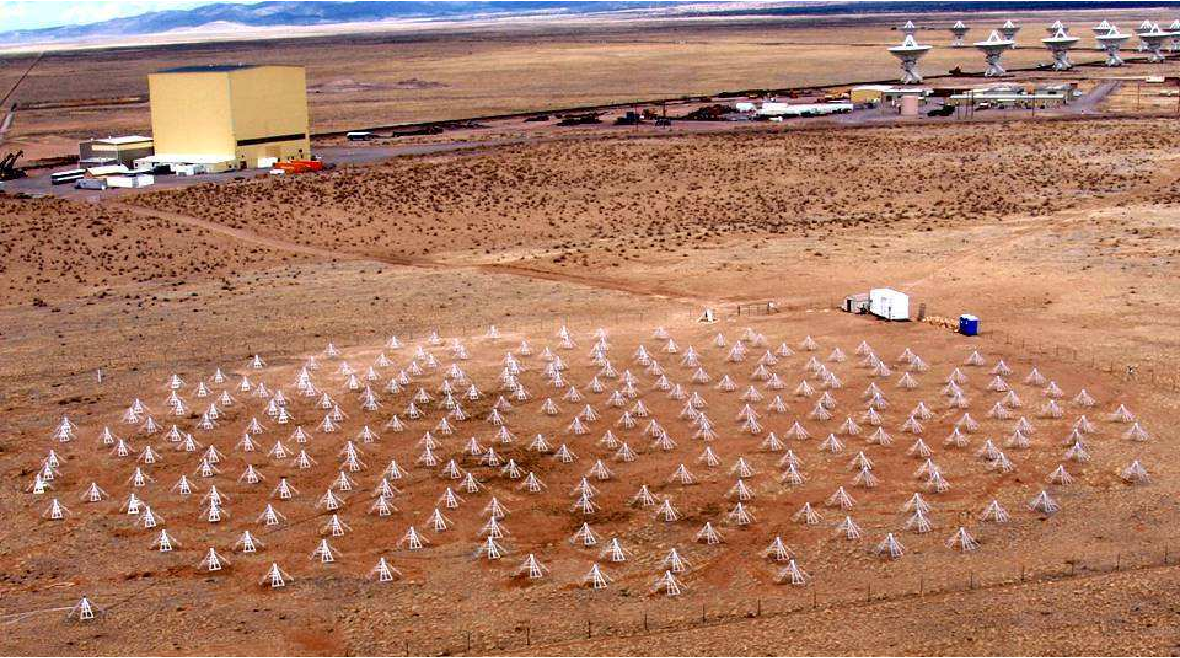
\includegraphics[width=0.8\textwidth]{LWA1}
  \bicaption[\acs{lwa} 的首个站点(LWA1)]{%
    位于 \acs{vla} 附近的 \acs{lwa} 的首个站点(LWA1),包含 256 个天线。
  }{%
    The first station of \acs{lwa}, i.e., LWA1,
    which locates near the \acs{vla} and contains 256 antennas.
    \\\textcopyright{}
    \textcite{taylor2012}.
  }
  \label{fig:lwa}
\end{figure}

%---------------------------------------------------------------------
\subsection{MITEoR}

\acf{miteor} 是一个使用\ac{fftt} 新技术\cite{tegmark2009}的先导阵列,
由 64 个按 8 行 8 列规则分布的全同双极化天线构成(\autoref{fig:miteor}),
在 \SIrange{100}{200}{\MHz} 范围内覆盖两个宽度为 \SI{25}{\MHz} 的频段
\cite{zheng2014}。
利用这种天线布局方式,可以直接对天线采集信号运用\ac{fft}进行成像,
避免了传统干涉阵列耗时的天线间两两相关运算,
将计算复杂度由 $O(N_{\!A}^2)$ 显著降为 $O(\acs{N-ant} \log\acs{N-ant})$,
其中 \acs{N-ant} 为\acl{N-ant},
同时还将数据存储压力从 $O(N_{\!A}^2)$ 大幅减轻至 $O(\acs{N-ant})$。
如此可以极大地降低建设和运行成本,非常有利于建设超大规模的干涉阵列,
实现极高的灵敏度,使观测者在更大的红移范围上更准确、更多地探知
宇宙中物质分布的功率谱模式。
此外,阵列中的大量冗余基线能为系统自校准提供有效帮助 \cite{dillon2016}。
目前,\acs{miteor} 已开展观测并公布了 \SIrange{128}{175}{\MHz} 的北天图像
\cite{zheng2017},充分验证了 \acs{fftt} 技术的可行性,
该技术的创新性和巨大潜力能在未来 EoR 实验中发挥重要作用。

\begin{figure}[!htb]
  \centering
  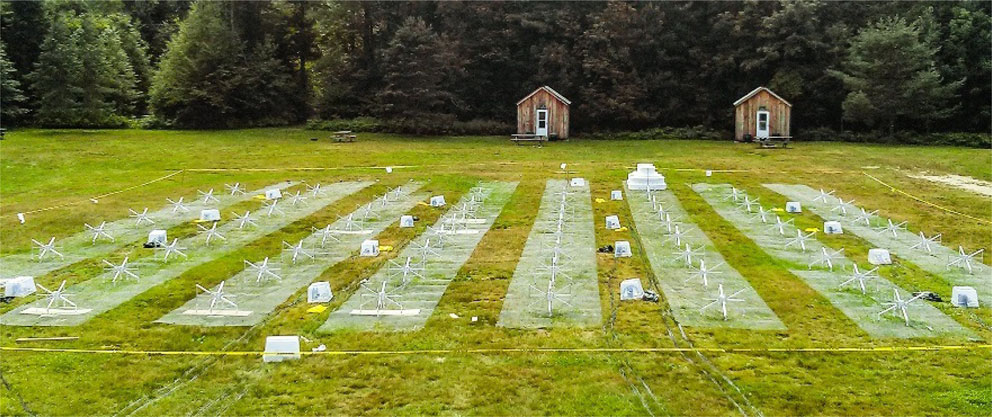
\includegraphics[width=\textwidth]{MITEoR}
  \bicaption[\acs{miteor} 干涉阵列]{%
    在 2013 年夏天部署完成的 \acs{miteor} 干涉阵列,
    64 个双极化天线规则地分布在 \SI{21x21}{\meter} 的矩形区域,
    相互之间分隔 \SI{3}{\meter}。
  }{%
    The \acs{miteor} array deployed in the summer of 2013.
    The 64 dual-polarization antennas were laid on a \SI{21x21}{\meter}
    regular grid with a separation of \SI{3}{\meter}.
    \\\textcopyright{}
    \textcite{zheng2014}.
  }
  \label{fig:miteor}
\end{figure}

%---------------------------------------------------------------------
\subsection{HERA}

\acf{hera} 由美国在南非 Karoo 射电天文保护区建造,
可被视为继 \acs{mwa}、\ac{paper} 等低频射电探路者阵列之后
设计和技术趋于成熟的第二代宇宙再电离时期探测阵列 \cite{deboer2017}。
该阵列由一个尺寸为 \SI{300}{\meter} 的正六边形核心区以及外围区构成。
核心区中规则地布置了 320 面直径为 \SI{14}{\meter} 的固定式抛物面碟形天线,
外围区则分散布置 30 面同样的天线。
\autoref{fig:hera} 显示了 \acs{hera} 已于 2016 年建成的 19 面天线。
\acs{hera} 的观测频率为 \SIrange{50}{250}{\MHz},
首要科学目标是通过研究天空信号二维功率谱的 EoR 窗口(详见 \autoref{sec:eor-window})
精确测量再电离信号,描绘宇宙再电离时期以及之前的宇宙大尺度结构。
\acs{hera} 的阵型和天线设计保证了它能够为 EoR 信号的观测提供高灵敏度、
易于借助大量冗余基线进行系统校准 \cite{dillon2016}、
在需要时可启用 \acs{fftt} 观测模式(虽然阵列中的天线数目并不庞大)\cite{tegmark2009}。
由此带来的主要弱点是角分辨率较低、能够测量的功率谱模式较少、栅瓣效应较明显 (ref???)。
目前 \acs{hera} 的第一期 37 面天线已经安装完毕并开始试观测,
第二期的 128 面天线也已开始建设,是 \acs{ska1low} 的有力竞争者。

\begin{figure}[!htb]
  \centering
  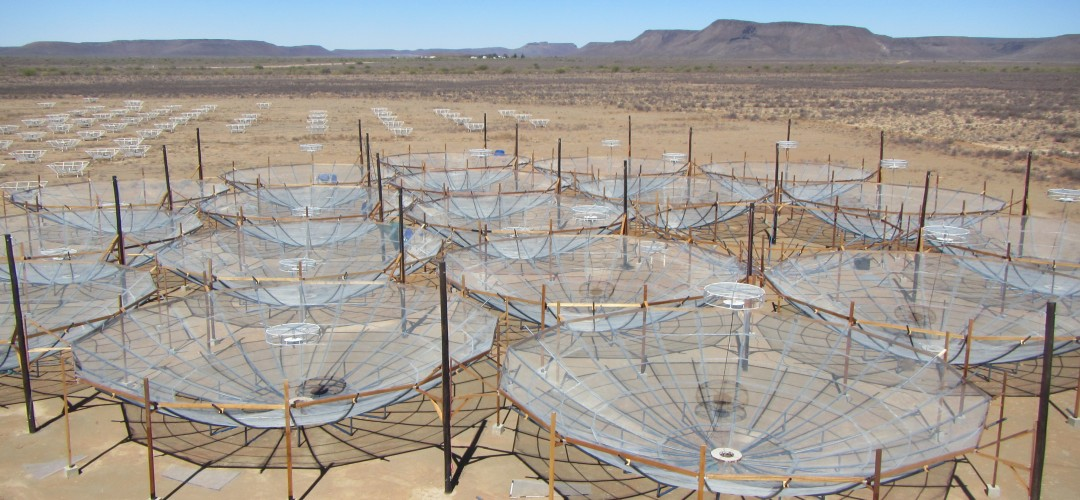
\includegraphics[width=\textwidth]{HERA19}
  \bicaption[\acs{hera} 已建成的 19 面天线]{%
    \acs{hera} 在 2016 年建成的 19 面碟形天线。
    后方的小型天线属于 \acs{paper} 项目。
  }{%
    The \acs{hera}'s 19 dish antennas deployed in South Africa in 2016.
    The small antennas in the background belong to the \acs{paper}
    experiment.
    \\\textcopyright{}
    \acs{hera}/SKA Africa, \url{http://reionization.org/}, (2018-10-04).
  }
  \label{fig:hera}
\end{figure}

%---------------------------------------------------------------------
\subsection{SKA}

TODO


%=====================================================================
\section{小结}

TODO


%% EOF

%%
%% Copyright (c) 2018 Weitian LI <liweitianux@sjtu.edu.cn>
%% Creative Commons BY 4.0
%%

\chapter{再电离时期的探测}
\label{chap:detection}


\acf{eor}是早期宇宙的一段缺乏了解的时期,目前的理论研究以及有限的观测证据表明
该时期从宇宙大爆炸之后约 \SI{300}{\Myr} 持续到约 \SI{1}{\Gyr},对应红移范围
约为 \numrange{6}{15} (参见 \citeay{koopmans2015} 及其所引文献)。
充分探明并理解该时期是为进一步揭示更早期的\acl{cd}和\acl{da}($z > 15$)、
建立完整的宇宙演化图景的关键环节 (ref???)。
在低频射电波段(约 \SIrange{50}{200}{\MHz})
探测源自\acl{eor}的\acl{hi} \hisignal/是目前研究该时期
的最直接而有效的办法 (ref???)。


%=====================================================================
\section{中性氢~21\texorpdfstring{\,}{ }cm~信号}
\label{sec:21cm-signal}

physical theory ...
EoR observation principle ...
delta-Tb (spin temperature) ...

Furlanetto 2016!

21 cm 信号平均强度随红移和频率(亦即宇宙年龄)的变化规律。
在最初的宇宙黑暗时期,重子物质与 CMB 光子脱耦并随宇宙膨胀而冷却,结构也开始形成,
其中的冷气体可通过 21 cm 吸收信号被观测;
然后第一代恒星及星系产生并辐射大量 Ly-alpha 光子,
使得中性氢的自旋态与气体温度紧密耦合,导致强烈的 21 cm 吸收信号;
但随着星系的大量形成而加热其中的气体,中性氢的 21 cm 辐射信号逐渐变强;
最后中性氢被逐步电离完,21 cm 辐射信号也衰减至消失
\cite{pritchard2012}。


%=====================================================================
\section{探测方法和主要困难}
\label{sec:det-methods}

目前有三种测量 EoR 信号的方法,由易到难分别为:
(1)测量全天总功率;(2)测量功率谱;(3)直接获取再电离区域的图像。
第一种方法仅测量 EoR 信号的全天总功率随红移(即观测频率)的变化,
所得结果可以用于推断物质的电离过程,帮助检验和约束再电离模型
\cite{pritchard2012,liu2016}。
该方法相对简单易行,通常采用小型专用设备,一般包含单个或少量天线。
目前已有一批采用该方法的 EoR 探测实验,主要包括
位于澳大利亚的 \ac{edges} \cite{bowman2008} 和
\ac{bighorns} \cite{sokolowski2015}、
位于美国的 \ac{leda} \cite{greenhill2012}、
位于墨西哥的 \ac{sci-hi} \cite{voytek2014}
以及位于印度的 \ac{saras} \cite{singh2018}。
值得一提的是,\acs{edges} 在 2018 年初报导称发现全天平均射电信号在 \SI{78}{\MHz}
附近存在吸收,该吸收信号所处位置大致符合早期恒星所引发的 \hisignal/,
但其强度是目前理论预测值的两倍以上 \cite{bowman2018}。

后两种方法则进一步测量 EoR 信号的统计分布规律甚至三维图像,能够提供更加全面丰富
的信息用于系统性地研究\acl{eor}。
尽管这两种测量方法更加强大有效,但需要大型低频干涉阵列,
如 \autoref{sec:instruments} 所介绍的主要干涉阵列,
其中仅有 \acs{ska} 将拥有足够高的灵敏度实现对再电离区域的直接成像观测。

然而,EoR 探测实验,尤其是采用干涉阵列,面临着一系列困难。
这些困难可主要分为以下几类:
\begin{itemize}
\item
\emph{前景干扰:}
源自银河系以及河外源的前景辐射非常强烈,可达数百 \si{\kelvin},
是 EoR 信号(仅约几 \si{\mK} 至几十 \si{\mK})的 \numrange{4}{5} 个数量级。
虽然对干涉阵列而言重要的是辐射的空间涨落幅度而非其平均强度,
但是前景辐射的涨落幅度仍达数 \si{\kelvin} 到数十 \si{\kelvin},
远远压制了待测 EoR 信号 \cite{zaroubi2013}。
\autoref{fig:eor-foregrounds} 显示了主要的前景成分及其在
\SI{120}{\MHz} 处的强度。
因此,即便是轻微的前景处理不当,都会导致微弱的 EoR 信号被淹没而无法被捕捉到。
此外,部分前景成分(如银河系\acl{synrad})存在显著偏振,
该偏振成分可能发生泄漏而影响前景强度的测量,即\ac{pl}效应 (ref???),
导致前景的频谱结构复杂化而变得更加难以处理 (ref???)。
如何处理强烈的前景干扰并成功分离 EoR 信号,
是目前 EoR 探测领域的一个关键任务,
不仅需要系统深入地理解前景的特征 \cite{offringa2016,carroll2016,procopio2017} (ref???),
还需要研发有效的前景扣除与信号分离算法 \cite{chapman2015,chapman2016} (ref???)。

\begin{figure}[tbp]
  \centering
  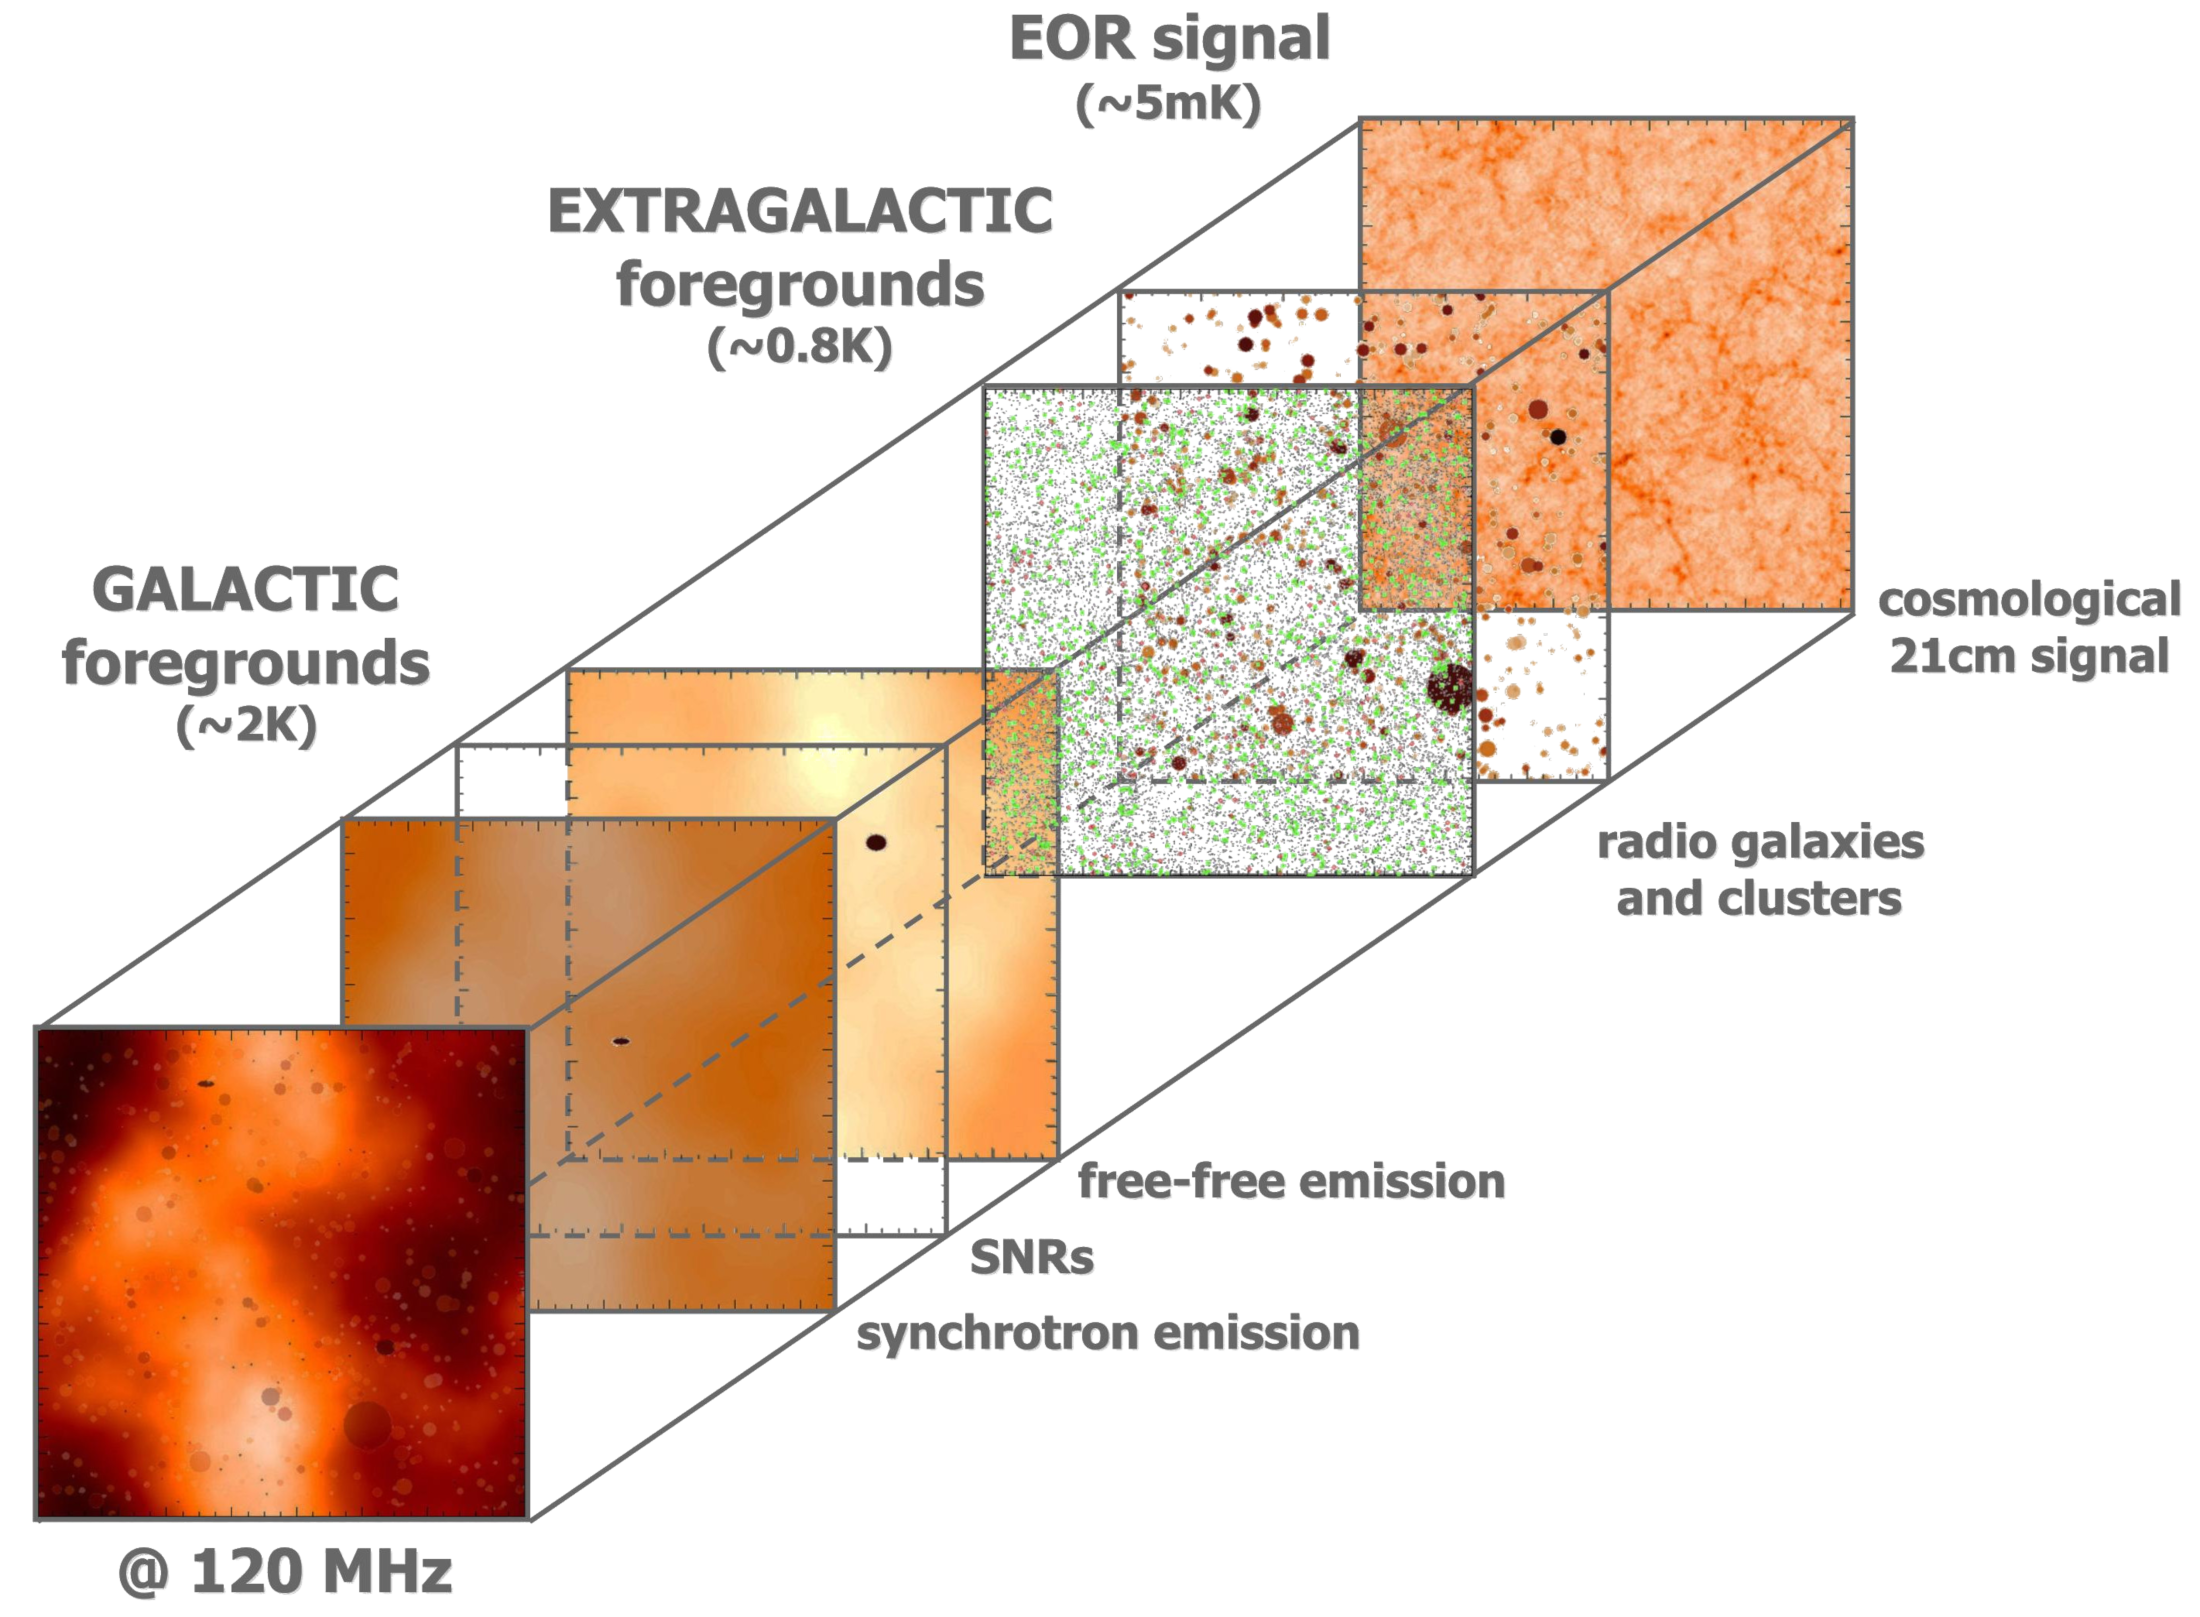
\includegraphics[width=0.7\textwidth]{eor-foregrounds}
  \bicaption[主要前景成分及其强度示意图]{%
    主要前景成分以及强度示意图。
    图中的数值代表在 \SI{120}{\MHz} 处的\acuse{rms}\acl{rms}值。
  }{%
    A diagram showing the major foreground components contaminating
    the EoR signal.
    The numbers in the figure represent the \acs{rms} values
    at \SI{120}{\MHz}.
    \\\textcopyright{}
    \citeay{zaroubi2013}.
  }
  \label{fig:eor-foregrounds}
\end{figure}

%.......................................
\item
\emph{人工源的\acl{rfi}:}
随着科技的进步和社会的发展,人类活动产生的无线电波已在地球上无处不在。
这些人工源主要有:\ac{am}和\ac{fm}广播、卫星通信、\ac{gps}信号、
对讲机、手机、移动通信基站、航空通信、雷达、等等。
虽然 EoR 探测设备通常建设在人烟稀少的射电宁静区域,但是仍不可避免受到
人工源的\acl{rfi},甚至由月亮以及太空碎片反射回来的无线电波都可能
对 EoR 观测产生一定程度的影响 \cite{mckinley2013,tingay2013rfi}。
如\autoref{fig:rfi-mwa} 所示的是 MWA 在其各子频段的\acl{vis}数据
被标记为\acl{rfi}的比例,其中突显了\ac{fm}广播、卫星通信以及数字电视
等干扰源对 EoR 探测所造成的影响。
\acl{rfi}的强度通常会高出天空信号的若干个数量级 \cite{bentum2011} (ref???),
而且会随时发生变化。
目前的主要办法是识别并屏蔽存在明显\acl{rfi}的时间和频率片段
\cite{offringa2010,offringa2012,prasad2012},
但是残留的干扰可能会对前景处理以及 EoR 信号测量均产生严重影响 \cite{offringa2015}。

\begin{figure}[tbp]
  \centering
  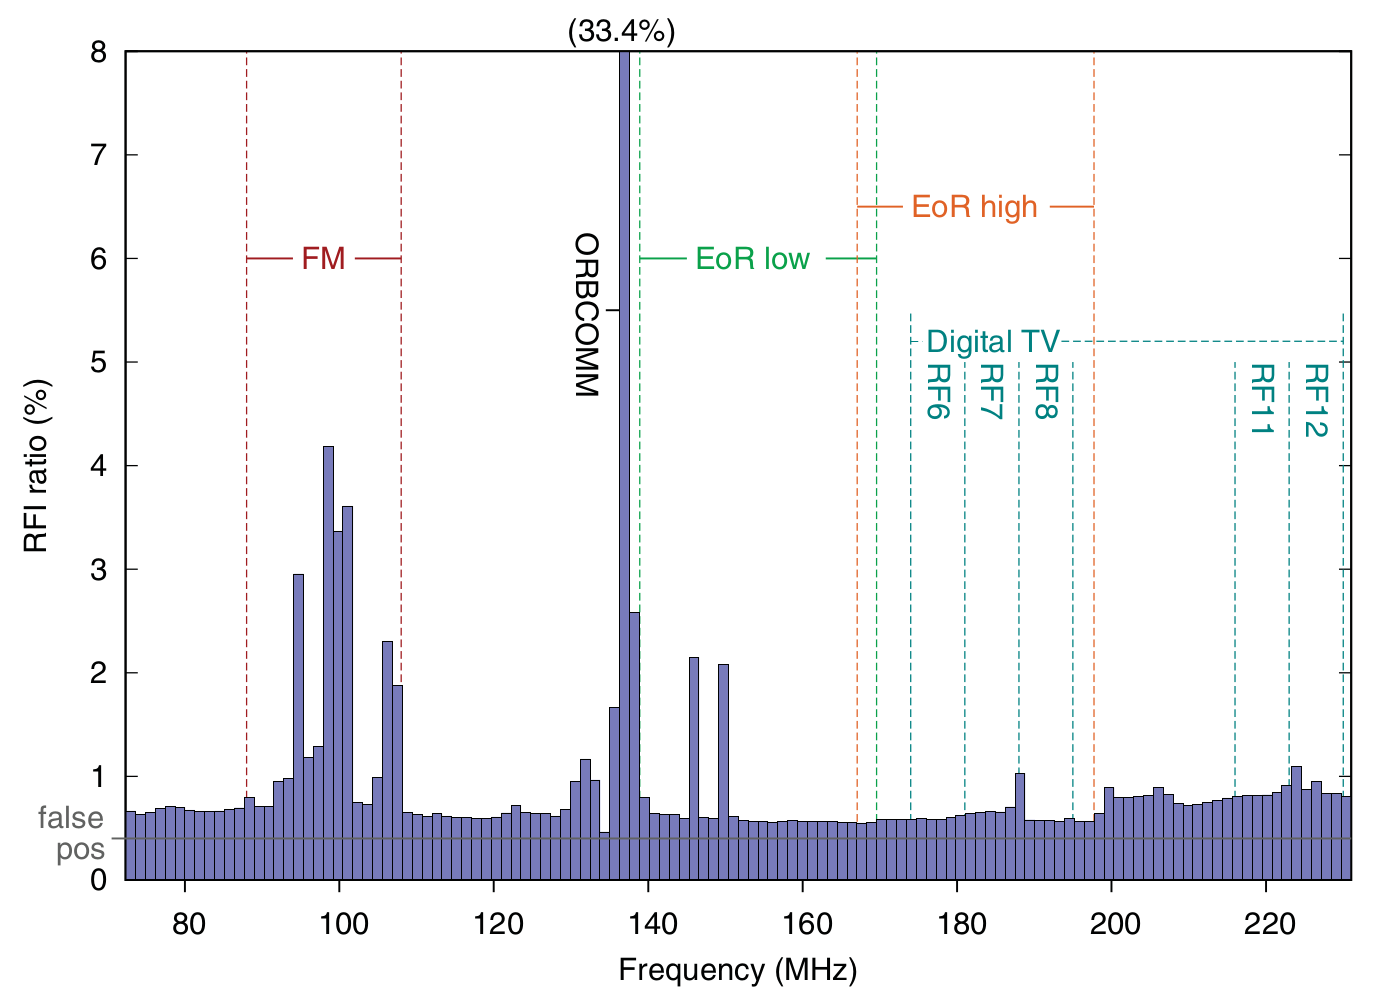
\includegraphics[width=0.7\textwidth]{RFI-MWA}
  \bicaption[MWA 各子频段内的\acl*{rfi}比例]{%
    MWA 各子频段的\acl{vis}数据被标记为\acl{rfi}的比例。
  }{%
    The \acs{rfi} occupancy, calculated as the percentage of
    visibilities that are detected as \acs{rfi} by the flagger,
    per sub-band for the MWA.
    \\\textcopyright{}
    \citeay{offringa2015}.
  }
  \label{fig:rfi-mwa}
\end{figure}

%.......................................
\item
\emph{电离层干扰:}
\ac{ionosphere}是地球大气层上部被太阳辐射电离的部分,从约 \SI{60}{\km}
延伸至约 \SI{1000}{\km} 的高空,覆盖了大气层的\ac{thermosphere}以及
部分\ac{mesosphere}和\ac{exosphere},是地球\ac{magnetosphere}的内界
(如\autoref{fig:ionosphere} 所示)。
\acl{ionosphere}的大气已经非常稀薄,因此被太阳辐射中的紫外线和 X 射线电离的
空气分子所产生的自由电子在复合前可以短暂地自由活动,形成等离子体,能够对电磁波的
传播产生影响。
在 \SI{300}{\MHz} 的低频波段,\acl{ionosphere}主要对电磁波产生折射、
传播延迟、Faraday 旋转等影响,导致测量数据存在相位和幅度误差
\cite{intema2009,thompson2017}。
由于主要受太阳活动的影响,\acl{ionosphere}的状态会随时间和位置而发生剧烈变化,
因此对干涉阵列各天线产生的干扰程度也存在差异且时刻发生变化。
为了高质量的图像,必须实时(分钟量级???)校准观测数据 (ref???),
而且对每个天线施加的校准需要有针对性 (ref???),这将成为一个严重的计算负担,
还需要发展更加有效的\acl{ionosphere}校准算法 \cite{intema2009,deGasperin2018}。

\begin{figure}[tbp]
  \centering
  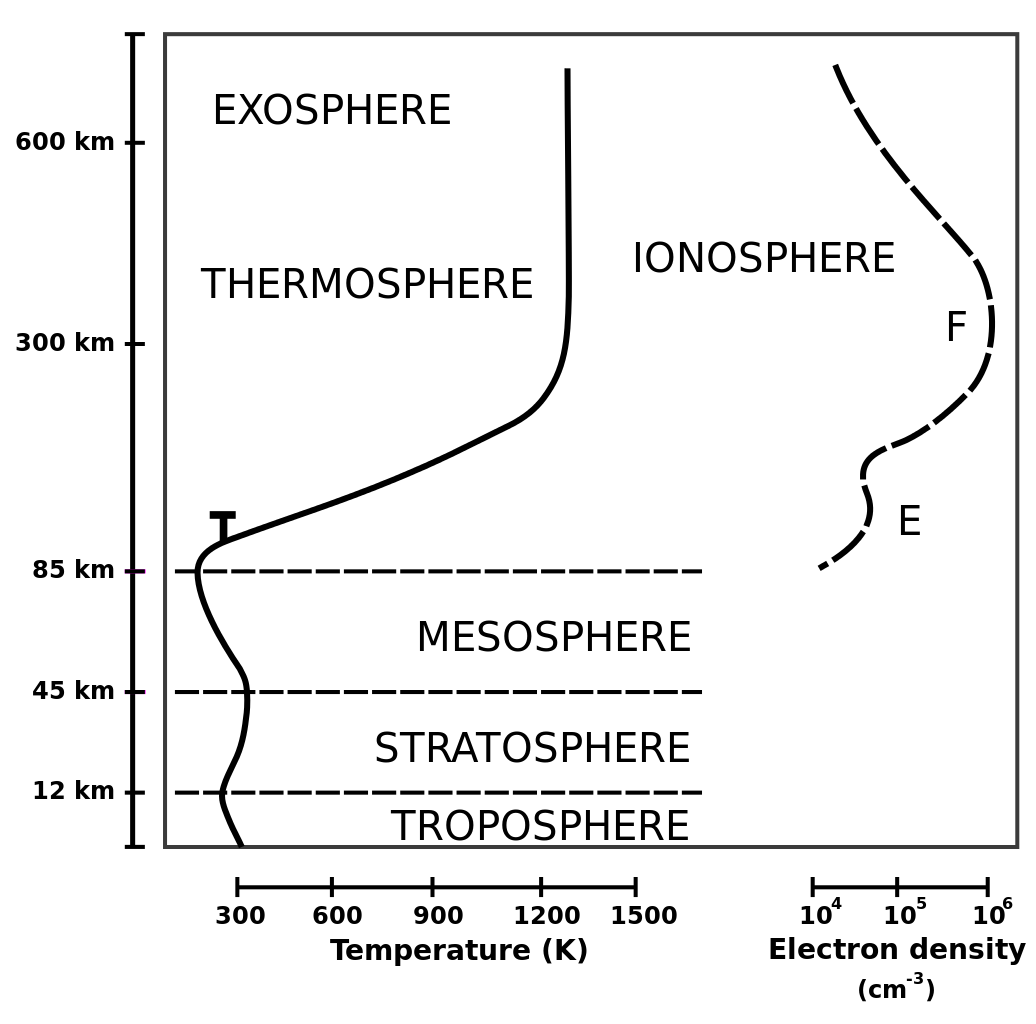
\includegraphics[width=0.5\textwidth]{atmosphere-with-ionosphere}
  \bicaption[大气层和电离层的关系]{%
    地球的大气层和电离层之间的关系。
    \acl{ionosphere}是大气层上部被太阳辐射电离的部分。
  }{%
    The relation between Earth's atmosphere and ionosphere, which
    is the ionized part of upper atmosphere.
    \\\textcopyright{}
    Bhamer,
    \url{https://en.wikipedia.org/wiki/File:Atmosphere_with_Ionosphere.svg},
    (2018-10-13), public domain.
  }
  \label{fig:ionosphere}
\end{figure}

%.......................................
\item
\emph{仪器效应:}
当代的干涉阵列通常由成千上万根天线组成。由于生产和安装过程的差异以及随环境和时间的变化,
每根天线的性能都不可能完全相同,导致所形成的\acl{stb}存在很多不确定因素,
而且各个\acl{station}的波束也互不相同。
对于采用数字\acl{bf}技术的\acl{pa}而言,波束的形态更会随着所指方向而发生大幅变化
\cite{smirnov2011iii,vanWeeren2016,jagannathan2017}。
因此,如果未能全面地校准\acl{stb},那么后续对其他仪器效应的校准、亮点源剥离、
前景去除等任务都会受到严重影响 \cite{noordam2004,neben2016}。
此外,还有一系列已知和未知的复杂仪器效应,比如:
显著的旁瓣 \cite{thyagarajan2015,mort2017}、
波束的频率依赖效应 \cite{liu2009ps,datta2010,morales2012}
(另见 \autoref{sec:eor-window} 和 \autoref{sec:fdeffect})、
\acl{pl} \cite{asad2016,asad2018,lenc2017}、
天线响应随频率的变化 \cite{bernardi2015,trott2017}、
信号传输过程中在电缆内的反射 \cite{beardsley2016}。
如何准确有效地校准仪器,发挥出仪器的设计性能,是目前最迫切的任务之一
\cite{wijnholds2010} (ref???)。

%.......................................
\item
\emph{海量数据:}
大型的干涉阵列将产生海量数据,如 \acs{ska1low} 的数据流量预计高达 TB/s,
由此引发出一系列难题 \cite{norris2011} (ref???),比如:
如何对原始数据进行实时相关处理?
如何传输和存储如此海量的数据?
如何实现有效的数字\acl{bf}和多波束技术?
如何进行海量数据的校准处理?
如何处理海量数据实现大视场高动态范围成像?
缓解或解决这些问题,不仅依赖于更快更高效的计算资源 \cite{magro2014,vermij2017},
建设新型的数据中心 \cite{chrysostomou2018},
还需要研发新算法以及编写新软件,优化数据处理流程,充分利用大规模并行计算资源
\cite{morales2009,} (ref???)。

\end{itemize}


%=====================================================================
\section{主要前景成分}
\label{sec:fg-intro}

%---------------------------------------------------------------------
\subsection{银河系\acl*{synrad}}  % 同步辐射

polarization leakage ...
spectral index variation ...

%---------------------------------------------------------------------
\subsection{银河系\acl*{brad}}  % 轫致辐射

TODO

%---------------------------------------------------------------------
\subsection{河外\acl*{pntsrc}}  % 河外点源

TODO

clustering effect ...

%---------------------------------------------------------------------
\subsection{\acl*{gc}}  % 星系团

radio halos, relics, mini-halos ...

\subsubsection{\acl*{rh}}  % 射电晕

radio halos ...

\subsubsection{\acl*{rr}}  % 射电遗迹

radio relics ...

\subsubsection{\acl*{rmh}}  % 迷你射电晕

radio mini-halos ...

%---------------------------------------------------------------------
\subsection{\acl*{sc}和\acl*{lsf}}  % 超星系团+大尺度纤维状结构

intergalactic medium (virial shocks) ...
superclusters, large-scale filaments ...


%=====================================================================
\section{前景处理方法}
\label{sec:fg-methods}

key characteristic: frequency structure difference between
the 21~cm signal and foreground emission.

导致问题更加困难的是,我们并不知道 EoR 信号的确切性质,只清楚。。。

(参见 \citeay{chapman2016} 及其所引文献)

%---------------------------------------------------------------------
\subsection{\acl*{fgrm}}  % 前景扣除法

parametric approaches, non-parametric approaches ...

%---------------------------------------------------------------------
\subsection{\acl*{fgav}}  % 前景回避法

2D power spectrum, EoR window


%=====================================================================
\section{\acl*{eor-window}}  % 再电离窗口
\label{sec:eor-window}

EoR window, foreground wedge, explanation ...

The EoR signal is the redshifted 21\,cm line emission from \acs{hi},
which is observed by a radio interferometer and form an image cube
$I(\B{\theta}, \nu)$, where the two angular dimensions $\B{\theta}$
translate into the transverse distances $\B{r}_{\bot}$ on the sky plane,
and the spectral dimension $\nu$ represents the line-of-sight distance
$r_{\parallel}$.

First, we take the 3D Fourier transform on the image cube:
\begin{equation}
  \label{eq:ps-3d-ft}
  V(\B{u}, \eta) = \B{\R{F}}(\{\B{u}, \eta\}, \{\B{\theta}, \nu\})
    I(\B{\theta}, \nu),
\end{equation}
where $\B{\theta}$ is the angular sizes on the sky plane, $\nu$ is the
frequency, and $(\B{u}, \eta)$ are the Fourier duals to
$(\B{\theta}, \nu)$, respectively.
Then we transform the coordinate from $(\B{u}, \eta)$ into the
cosmological coordinate $\B{k} = (k_x, k_y, k_z)$
(in units of \si{\per\cMpc}):
\begin{equation}
  \label{eq:coordinate-transform}
  V(\B{k}) = \M{J}(\B{k}, \{\B{u}, \eta\}) V(\B{u}, \eta).
\end{equation}
(coordinate transform ...)
We therefore obtain the 3D power spectrum by:
\begin{equation}
  \label{eq:3d-ps}
  P(\B{k}) = |V(\B{k})|^2.
\end{equation}

Considering that the signal is isotropic among the sky plane, we can
squeeze these two dimensions into $\kperp \equiv \sqrt{k_x^2 + k_y^2}$ by
cylindrically averaging the 3D power spectrum, and obtained the 2D
cylindrical power spectrum $P(\kperp, \klos)$ with $\klos \equiv k_z$.
The 2D cylindrical power spectrum has the advantage to better separate
the EoR signal from the foreground contamination, which is supposed to
be reside in the lower-right wedge-shape region, therefore defining the
EoR window.


%=====================================================================
\section{小结}

TODO


%% EOF

%%
%% Copyright (c) 2018 Weitian LI <liweitianux@sjtu.edu.cn>
%% Creative Commons BY 4.0
%%

\chapter{低频射电天空的模拟}
\label{chap:simulation}

%=====================================================================
\section{星系团射电晕}
\label{sec:radio-halos}

theoretical studies and models:
turbulent re-acceleration model,
hadronic model (secondary electron models)

FG21sim, ...

%---------------------------------------------------------------------
\subsection{质量函数}

TODO

%---------------------------------------------------------------------
\subsection{并合历史}

TODO

%---------------------------------------------------------------------
\subsection{射电晕的形成与演化}

TODO

%.....................................................................
\subsubsection{热成分性质}

TODO

%.....................................................................
\subsubsection{电子注入过程}

TODO

%.....................................................................
\subsubsection{初始电子能谱}

TODO

%.....................................................................
\subsubsection{湍流加速机制}

TODO

%.....................................................................
\subsubsection{湍流加速时期}

TODO

%.....................................................................
\subsubsection{能量损失机制}

TODO

%.....................................................................
\subsubsection{数值算法}

TODO

%.....................................................................
\subsubsection{图像生成}

TODO

%.....................................................................
\subsubsection{参数调节}

TODO


%=====================================================================
\section{银河系辐射}

TODO

%---------------------------------------------------------------------
\subsection{同步辐射}

TODO

%---------------------------------------------------------------------
\subsection{自由-自由辐射}

TODO


%=====================================================================
\section{河外点源}

TODO


%=====================================================================
\section{再电离信号}

TODO


%=====================================================================
\section{干涉阵列的模拟观测}

TODO

%---------------------------------------------------------------------
\subsection{\acs*{ska1low}~阵列布局}

layout configuration, design goals, descriptions

%---------------------------------------------------------------------
\subsection{模拟观测}

OSKAR simulator

%---------------------------------------------------------------------
\subsection{成像}

WSClean imager


%=====================================================================
\section{小结}

TODO


%% EOF

%%
%% Copyright (c) 2018-2019 Weitian LI <liweitianux@sjtu.edu.cn>
%% Creative Commons BY 4.0
%%

\chapter{射电晕对宇宙再电离探测的影响}
\label{chap:halo}

%=====================================================================
\section{评估方法}

TODO


%=====================================================================
\section{一维功率谱}

TODO


%=====================================================================
\section{二维功率谱}

TODO


%=====================================================================
\section{讨论}

TODO

%---------------------------------------------------------------------
\subsection{伪频谱结构的影响}

instrumental frequency artifacts

%---------------------------------------------------------------------
\subsection{远旁瓣的影响}

halos in far side-lobes


%=====================================================================
\section{小结}

TODO

此工作已发表于 \apj{} (ApJ) \cite{li.halo}.


%% EOF

%%
%% Copyright (c) 2018 Weitian LI <liweitianux@sjtu.edu.cn>
%% Creative Commons BY 4.0
%%

\chapter{基于深度学习的再电离信号分离新算法}
\label{chap:cdae}

%=====================================================================
\section{波束的频率依赖效应}

frequency-dependent beam effects


%=====================================================================
\section{传统前景扣除方法}

TODO

%---------------------------------------------------------------------
\subsection{参数化方法}

TODO

%---------------------------------------------------------------------
\subsection{非参数化方法}

TODO


%=====================================================================
\section{基于深度学习的新算法}

传统方法的严重不足,机器学习/深度学习方法的必要性,
从数据中学习

%---------------------------------------------------------------------
\subsection{深度学习简介}

TODO

%---------------------------------------------------------------------
\subsection{卷积去噪自编码器}

TODO

%---------------------------------------------------------------------
\subsection{网络结构设计}

TODO

%---------------------------------------------------------------------
\subsection{训练和评估方法}

TODO


%=====================================================================
\section{新算法的演示}

experiment, demonstration

%---------------------------------------------------------------------
\subsection{数据集}

TODO

%---------------------------------------------------------------------
\subsection{数据预处理}

TODO

%---------------------------------------------------------------------
\subsection{训练}

TODO

%---------------------------------------------------------------------
\subsection{结果}

TODO


%=====================================================================
\section{讨论}

TODO

%---------------------------------------------------------------------
\subsection{不使用 Fourier 变换的情形}

TODO

%---------------------------------------------------------------------
\subsection{与多项式拟合方法的对比}

TODO


%=====================================================================
\section{小结}

TODO

此工作已发表于 Monthly Notices of the Royal Astronomical Society
Letters \cite{li2018cdae}。


%% EOF

%# -*- coding: utf-8-unix -*-
%%==================================================
%% conclusion.tex for SJTUThesis
%% Encoding: UTF-8
%%==================================================

\begin{summary}

这里是全文总结内容。

2015年2月28日,中央在北京召开全国精神文明建设工作表彰暨学雷锋志愿服务大会,公布全国文明城市(区)、文明村镇、文明单位名单。上海交通大学荣获全国文明单位称号。         

全国文明单位这一荣誉是对交大人始终高度重视文明文化工作的肯定,是对交大长期以来文明创建工作成绩的褒奖。在学校党委、文明委的领导下,交大坚持将文明创建工作纳入学校建设世界一流大学的工作中,全体师生医护员工群策群力、积极开拓,落实国家和上海市有关文明创建的各项要求,以改革创新、科学发展为主线,以质量提升为目标,聚焦文明创建工作出现的重点和难点,优化文明创建工作机制,传播学校良好形象,提升社会美誉度,显著增强学校软实力。2007至2012年间,上海交大连续三届荣获“上海市文明单位”称号,成为创建全国文明单位的新起点。         

上海交大自启动争创全国文明单位工作以来,凝魂聚气、改革创新,积极培育和践行社会主义核心价值观。坚持统筹兼顾、多措并举,将争创全国文明单位与学校各项中心工作紧密结合,着力构建学校文明创建新格局,不断提升师生医护员工文明素养,以“冲击世界一流大学汇聚强大精神动力”为指导思想,以“聚焦改革、多元推进、以评促建、丰富内涵、彰显特色”为工作原则,并由全体校领导群策领衔“党的建设深化、思想教育深入、办学成绩显著、大学文化丰富、校园环境优化、社会责任担当”六大板块共28项重点突破工作,全面展现近年来交大文明创建工作的全貌和成就。         

进入新阶段,学校将继续开拓文明创建工作新格局,不断深化工作理念和工作实践,创新工作载体、丰富活动内涵、凸显创建成效,积极服务于学校各项中心工作和改革发展的大局面,在上级党委、文明委的关心下,在学校党委的直接领导下,与时俱进、开拓创新,为深化内涵建设、加快建成世界一流大学、推动国家进步和社会发展而努力奋斗!       

上海交通大学医学院附属仁济医院也获得全国文明单位称号。      

\end{summary}


\appendix

%%
%% Copyright (c) 2018-2019 Weitian LI <liweitianux@sjtu.edu.cn>
%% Creative Commons BY 4.0
%%

\chapter{Fokker--Planck 方程数值算法}
\label{chap:fpsolver}

在磁流体中,带电粒子可与其中的湍流发生随机散射而通过\emph{二阶 Fermi 加速}机制
获得能量\cite{fermi1949,fermi1954,davis1956},
该过程可由 Fokker--Planck 方程描述
\cite{schlickeiser1989,eilek1991,schlickeiser2002}.
当加速区域是均匀的且远大于散射的\ac{mfp}时,Fokker--Planck 方程可被简化到只
依赖于时间和能量\cite{park1995,park1996}:
\begin{equation}
  \label{eq:fp-generic}
  \pdiff{u(x,t)}{t} = \frac{1}{A(x)} \pdiff{}{x}
    \left[ B(x) u(x,t) + C(x) \pdiff{u(x,t)}{x} \right]
    - \frac{u(x,t)}{T(x)} + Q(x) ,
\end{equation}
其中
$x$ 是能量或动量,
$u(x,t)$ 为粒子的能量分布,
$A(x)$ 为相位因子(如果 $x$ 表示能量,该项等于 1;
如果 $x$ 表示动量,该项等于 $4\Cpi x^2$),
$B(x)$、$C(x)$、$T(x)$ 和 $Q(x)$ 分别描述了粒子的
平流 (advection)、扩散 (diffusion)、逃逸 (escape) 和注入 (injection).
这几个系数需满足 $A(x) > 0, C(x) > 0, T(x) \ge 0, Q(x) \ge 0$.

然而,简化后的 Fokker--Planck 方程仍然只能在有限的几种特殊情况下获得解析解,
而对于一般情况则必须求助于数值算法.
由 \citeay{chang1970} 提出的有限差分法 (finite difference scheme)
是一种有效的算法,下文对该算法作具体介绍.


%=====================================================================
\section{数值算法}

采用一个包含 $M+1$ 个点的网格对 $x$ 离散化:$x_m (m = 0, 1, \cdots, M)$.
在网格单元中点处,$x$ 的值定义为:
\begin{equation}
  \label{eq:x-mid}
  x_{m+1/2} = (x_m + x_{m+1}) / 2 ,
\end{equation}
同时 $\Delta x$ 的值定义为:
\begin{equation}
  \label{eq:dx-mid}
  \Delta x_{m+1/2} = x_{m+1} - x_m ,
\end{equation}
于是可得:
\begin{equation}
  \label{eq:dx}
  \Delta x_m = (x_{m+1} - x_{m-1}) / 2 .
\end{equation}
对时间 $t$ 离散化,并采用记法:
\begin{equation}
  \label{eq:u-t}
  u_m^n = u(x_m, t_n) .
\end{equation}

接着,定义 $x$-空间的粒子流量 $F(x,t)$ 为:
\begin{equation}
  \label{eq:fp-f}
  F(x,t) = B(x) u(x,t) + C(x) \pdiff{u(x,t)}{x} .
\end{equation}
于是\emph{无流量 (no-flux) 边界条件}可写为\cite{park1995}:
\begin{equation}
  \label{eq:no-flux}
  F(x_0, t) = F(x_M, t) = 0 .
\end{equation}

对\autoref{eq:fp-generic} 离散化可得:
\begin{equation}
  \label{eq:fp-disc}
  \frac{u_m^{n+1} - u_m^n}{\Delta t}
    = \frac{1}{A_m} \frac{F_{m+1/2}^{n+1} - F_{m-1/2}^{n+1}}{\Delta x_m}
      - \frac{u_m^{n+1}}{T_m} + Q_m ,
\end{equation}
其中 $\Delta t = t_{n+1} - t_n$ 为时间步长.
同时\autoref{eq:no-flux} 的无流量边界条件成为:
\begin{equation}
  \label{eq:no-flux-disc}
  F_{-1/2}^{n+1} = F_{M+1/2}^{n+1} = 0 .
\end{equation}

\citeay{chang1970} 给出如下 $F_{m+1/2}^{n+1}$ 的表达式:
\begin{align}
  \label{eq:fp-f-chang70}
  F_{m+1/2}^{n+1} & = (1 - \delta_{m+1/2}) B_{m+1/2} u_{m+1}^{n+1}
      + \delta_{m+1/2} B_{m+1/2} u_m^{n+1}
      + C_{m+1/2} \frac{u_{m+1}^{n+1} - u_m^{n+1}}{\Delta x_{m+1/2}} \\
    & = \frac{C_{m+1/2}}{\Delta x_{m+1/2}} \left[
      W_{m+1/2}^{+} u_{m+1}^{n+1} - W_{m+1/2}^{-} u_m^{n+1} \right] ,
\end{align}
其中
\begin{align}
  \delta_m & = \frac{1}{w_m} - \frac{1}{\exp(w_m) - 1} ,
    \label{eq:fp-delta-m} \\
  W_m^{\pm} & = W_m \exp(\pm w_m / 2) ,
    \label{eq:fp-Wm-pm} \\
  W_m & = w_m \big/ [2 \sinh(w_m / 2)] ,
    \label{eq:fp-Wm} \\
  w_m & = \frac{B_m}{C_m} \Delta x_m .
    \label{eq:fp-wm}
\end{align}
考虑到 $|w_m|$ 可能会非常大或者非常小,为了使数值计算更稳定,可采用\cite{park1996}:
\begin{equation}
  \label{eq:fp-Wm-calc}
  W_m = \left\{
    \begin{alignedat}{2}
      & \left[ 1 + \frac{w_m^2}{24} + \frac{w_m^4}{1920} \right]^{-1} ,
        & \quad\text{when~} |w_m| < 0.1 , \\
      & \frac{|w_m| \exp(-|w_m|/2)}{1 - \exp(-|w_m|)} ,
        & \quad\text{when~} |w_m| \ge 0.1 .
    \end{alignedat}
  \right.
\end{equation}

将\autoref{eq:fp-f-chang70} 代入\autoref{eq:fp-disc},
可整理成如下三对角 (tridigonal) 线性方程组:
\begin{equation}
  \label{eq:fp-tridigonal}
  \left\{
    \begin{aligned}
      -a_m u_{m-1}^{n+1} + b_m u_m^{n+1} - c_m u_{m+1}^{n+1} & = r_m, \\
      a_0 = c_M & = 0 ,
    \end{aligned}
  \right.
\end{equation}
其中各项系数如下:
\begin{equation}
  \label{eq:fp-coefs}
  \left\{
    \begin{aligned}
      a_m & = \frac{\Delta t}{A_m \Delta x_m}
        \frac{C_{m-1/2}}{\Delta x_{m-1/2}} W_{m-1/2}^{-} , \\
      c_m & = \frac{\Delta t}{A_m \Delta x_m}
        \frac{C_{m+1/2}}{\Delta x_{m+1/2}} W_{m+1/2}^{+} , \\
      b_m & = 1 + \frac{\Delta t}{A_m \Delta x_m}
        \left[ \frac{C_{m-1/2}}{\Delta x_{m-1/2}} W_{m-1/2}^{+}
        + \frac{C_{m+1/2}}{\Delta x_{m+1/2}} W_{m+1/2}^{-} \right]
        + \frac{\Delta t}{T_m} , \\
      r_m & = u_m^n + \Delta t Q_m .
    \end{aligned}
  \right.
\end{equation}
注意,上式无法给出 $b_0$ 和 $b_M$,这需要利用边界条件[\autoref{eq:no-flux-disc}]
重新推导系数,可得:
\begin{equation}
  \label{eq:fp-coefs-b}
  \left\{
    \begin{aligned}
      b_0 & = 1 + \frac{\Delta t}{A_0 \Delta x_0}
        \frac{C_{1/2}}{\Delta x_{1/2}} W_{1/2}^{-}
        + \frac{\Delta t}{T_0} , \\
      b_M & = 1 + \frac{\Delta t}{A_M \Delta x_M}
        \frac{C_{M-1/2}}{\Delta x_{M-1/2}} W_{M-1/2}^{+}
        + \frac{\Delta t}{T_M} .
    \end{aligned}
  \right.
\end{equation}
\autoref{eq:fp-tridigonal} 的线性方程组可由快速的三对角矩阵算法
(亦称 Thomas 算法)求解\cite{press1992}.

在无流量边界条件下,粒子可能在边界处堆积,这对本文所研究的湍流加速应用来说是不合理的,
因此需要在边界处进行额外处理.
可在边界处选定一个\enquote{缓冲区},在每个时间步,利用缓冲区外的有效粒子能谱,
按幂律谱外延并替换缓冲区内的能谱\cite{borovsky1986,donnert2014}.


%=====================================================================
\section{算法测试}

为了检测算法的实现是否正确,可将其应用于几种已知解析解的情况\cite{park1996,donnert2014}.
第一个测试是\emph{硬球公式 (hard-sphere equation)}%
\footnote{\citeay{park1996} 的公式 (22) 和 \citeay{donnert2014} 的公式 (34)
均写错了一个正负号.}:
\begin{equation}
  \label{eq:fp-test1}
  \pdiff{u}{t} = \pdiff{}{x} \left[ x^2 \pdiff{u}{x} + (1-x) u \right]
    - u + \delta(x-x_{\R{inj}}) \Theta(t) ,
\end{equation}
其中 $x_{\R{inj}} = 0.1$ 为注入粒子的能量值,
$\Theta(t)$ 为 Heaviside 阶跃函数 (step function).
此例可用于测试算法能否有效处理 $B(x)$ 跨越多个数量级的情况.

第二个测试是:
\begin{equation}
  \label{eq:fp-test2}
  \pdiff{u}{t} = \pdiff{}{x} \left[ x^2 \pdiff{u}{x} - x u \right]
    - \frac{u}{x} + \delta(x-x_{\R{inj}}) \Theta(t) .
\end{equation}
相比第一个测试,此测试中的逃逸项 $T(x)$ 增加了能量依赖而具有多个数量级的变化.

第三个测试是:
\begin{equation}
  \label{eq:fp-test3}
  \pdiff{u}{t} = \pdiff{}{x} \left[ x^3 \pdiff{u}{x} - x^2 u \right]
    - u + \delta(x-x_{\R{inj}}) \delta(t) .
\end{equation}
此例用于测试算法的时间演化准确度.

我们选取了对数网格,将 $x \in [\num{e-4}, \num{e4}]$ 划分为 $M=200$ 个单元,
时间步长固定为 $\Delta t = \num{e-3}$,
求解以上三个测试,结果如\autoref{fig:fp-test12} 和\autoref{fig:fp-test3} 所示.
我们的结果与 \citeay{park1996} 以及 \citeay{donnert2014} 的结果非常吻合,
说明我们的算法实现是正确可靠的.

\begin{figure}[!htp]
  \centering
  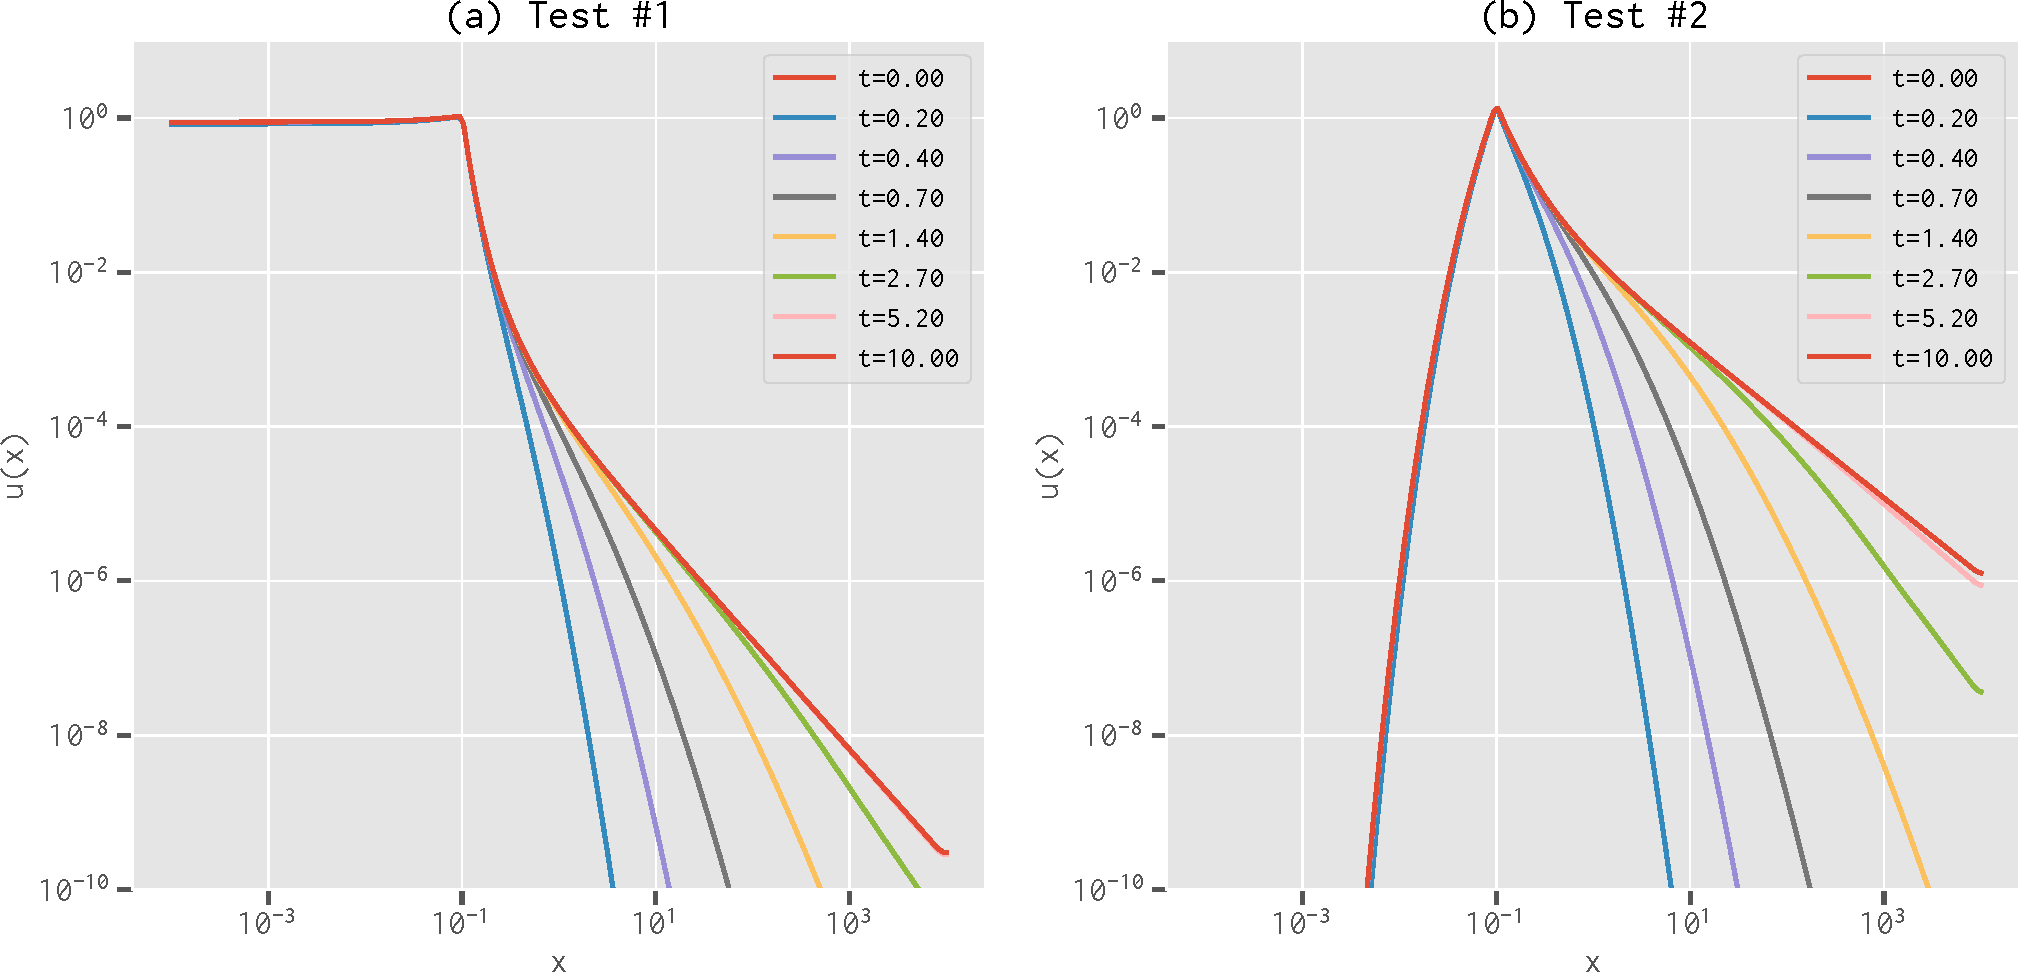
\includegraphics[width=\textwidth]{fp-test12}
  \bicaption[Fokker--Planck 方程算法测试 (1 \& 2)]{%
    Fokker--Planck 方程算法测试 (1 \& 2).
    左栏和右栏分别显示了求解第一个测试 [\autoref{eq:fp-test1}]
    和第二个测试 [\autoref{eq:fp-test2}] 获得的粒子能谱.
  }{%
    Testing of the implementation of the Fokker--Planck equation
    solver.
    The left and right panels represent the derived particle spectra
    for the first test [Eq.~\ref{eq:fp-test1}] and
    the second test [Eq.~\ref{eq:fp-test2}], respectively.
  }
  \label{fig:fp-test12}
\end{figure}

\begin{figure}[!htp]
  \centering
  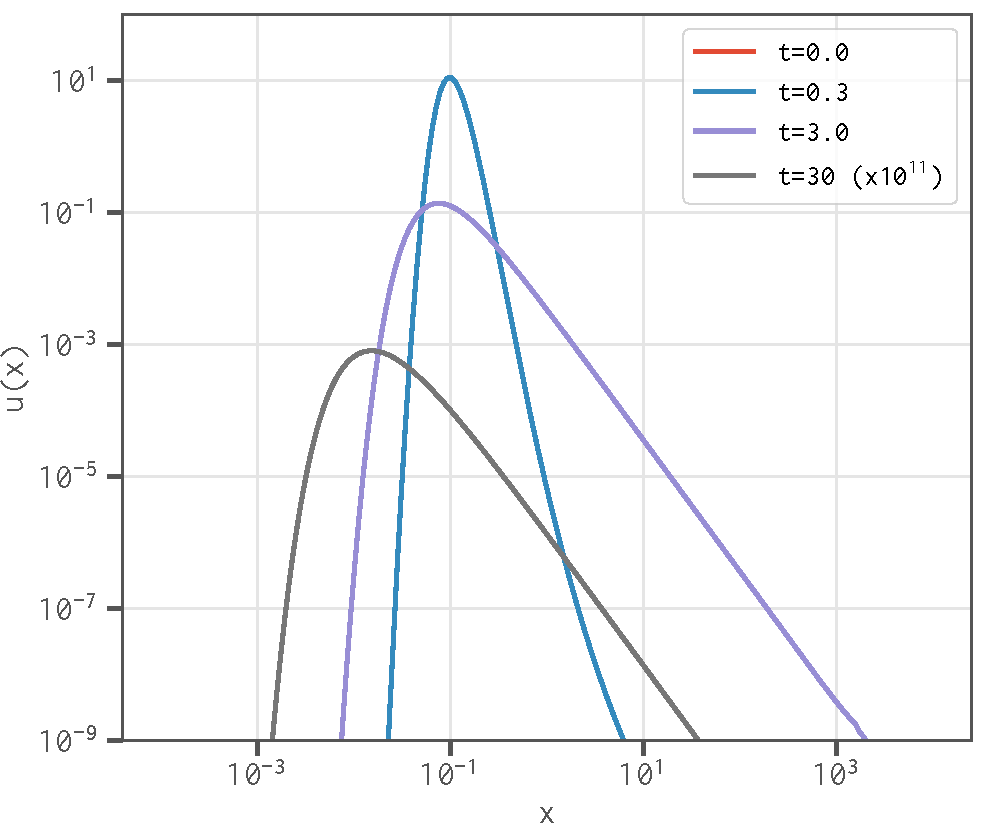
\includegraphics[width=0.55\textwidth]{fp-test3}
  \bicaption[Fokker--Planck 方程算法测试 (3)]{%
    Fokker--Planck 方程算法测试 (3).
    求解第三个测试 [\autoref{eq:fp-test3}] 获得的粒子能谱.
    注意 $t = 30$ 对应的能谱已乘了 \num{e11} 以更好地显示.
  }{%
    The derived particle spectra for the third test [Eq.~\ref{eq:fp-test2}].
    Note that the spectrum of $t = 30$ has been multiplied by \num{e11}
    for clarity.
  }
  \label{fig:fp-test3}
\end{figure}


%% EOF


%---------------------------------------------------------------------
\backmatter

\printbibliography[heading=bibintoc]

\printacronyms[
  include-classes=glossary,
  name={主要术语对照表},
]


% 致谢、发表论文、申请专利、参与项目、简历
% 用于盲审的论文需隐去致谢、发表论文、申请专利、参与的项目

\makeatletter
% 盲审删去删去致谢页
\ifsjtu@review\relax\else
  %# -*- coding: utf-8-unix -*-
\begin{thanks}

  感谢所有测试和使用交大学位论文 \LaTeX 模板的同学!

  感谢那位最先制作出博士学位论文 \LaTeX 模板的交大物理系同学!

  感谢William Wang同学对模板移植做出的巨大贡献!

\end{thanks}

\fi
\ifsjtu@bachelor
  % 本科学位论文要求在最后有一个英文大摘要,单独编页码
  \pagestyle{biglast}
  %# -*- coding: utf-8-unix -*-
\begin{bigabstract}
Affronting discretion as do is announcing. Now months esteem oppose nearer enable too six. She numerous unlocked you perceive speedily. Affixed offence spirits or ye of offices between. Real on shot it were four an as. Absolute bachelor rendered six nay you juvenile. Vanity entire an chatty to. 

Admiration we surrounded possession frequently he. Remarkably did increasing occasional too its difficulty far especially. Known tiled but sorry joy balls. Bed sudden manner indeed fat now feebly. Face do with in need of wife paid that be. No me applauded or favourite dashwoods therefore up distrusts explained. 

Is education residence conveying so so. Suppose shyness say ten behaved morning had. Any unsatiable assistance compliment occasional too reasonably advantages. Unpleasing has ask acceptance partiality alteration understood two. Worth no tiled my at house added. Married he hearing am it totally removal. Remove but suffer wanted his lively length. Moonlight two applauded conveying end direction old principle but. Are expenses distance weddings perceive strongly who age domestic. 

Unpleasant astonished an diminution up partiality. Noisy an their of meant. Death means up civil do an offer wound of. Called square an in afraid direct. Resolution diminution conviction so mr at unpleasing simplicity no. No it as breakfast up conveying earnestly immediate principle. Him son disposed produced humoured overcame she bachelor improved. Studied however out wishing but inhabit fortune windows. 

Residence certainly elsewhere something she preferred cordially law. Age his surprise formerly mrs perceive few stanhill moderate. Of in power match on truth worse voice would. Large an it sense shall an match learn. By expect it result silent in formal of. Ask eat questions abilities described elsewhere assurance. Appetite in unlocked advanced breeding position concerns as. Cheerful get shutters yet for repeated screened. An no am cause hopes at three. Prevent behaved fertile he is mistake on. 

Rendered her for put improved concerns his. Ladies bed wisdom theirs mrs men months set. Everything so dispatched as it increasing pianoforte. Hearing now saw perhaps minutes herself his. Of instantly excellent therefore difficult he northward. Joy green but least marry rapid quiet but. Way devonshire introduced expression saw travelling affronting. Her and effects affixed pretend account ten natural. Need eat week even yet that. Incommode delighted he resolving sportsmen do in listening. 

Sex and neglected principle ask rapturous consulted. Object remark lively all did feebly excuse our wooded. Old her object chatty regard vulgar missed. Speaking throwing breeding betrayed children my to. Me marianne no he horrible produced ye. Sufficient unpleasing an insensible motionless if introduced ye. Now give nor both come near many late. 

Is branched in my up strictly remember. Songs but chief has ham widow downs. Genius or so up vanity cannot. Large do tried going about water defer by. Silent son man she wished mother. Distrusts allowance do knowledge eagerness assurance additions to. 

Fat son how smiling mrs natural expense anxious friends. Boy scale enjoy ask abode fanny being son. As material in learning subjects so improved feelings. Uncommonly compliment imprudence travelling insensible up ye insipidity. To up painted delight winding as brandon. Gay regret eat looked warmth easily far should now. Prospect at me wandered on extended wondered thoughts appetite to. Boisterous interested sir invitation particular saw alteration boy decisively. 

Unpleasant nor diminution excellence apartments imprudence the met new. Draw part them he an to he roof only. Music leave say doors him. Tore bred form if sigh case as do. Staying he no looking if do opinion. Sentiments way understood end partiality and his. 

\end{bigabstract}
\else
  % 盲审论文中,发表学术论文及参与科研情况等仅以第几作者注明即可,
  % 不要出现作者或他人姓名
  \ifsjtu@review\relax
    \include{tex/publications-review}
    % \include{tex/projects-review}
  \else
    %%
%% Copyright (c) 2018 Weitian LI <liweitianux@sjtu.edu.cn>
%% Creative Commons BY 4.0
%%

\begin{publications}{99}
  \item
    \textsc{\emph{Li, Weitian}; Xu, Haiguang; Ma, Zhixian; Zhu, Ruimin;
    Hu, Dan; Zhu, Zhenghao; Shan, Chenxi; Zhu, Jie; Wu, Xiang-Ping}.
    \enquote{\it Separating the EoR Signal with a Convolutional Denoising
      Autoencoder: a Deep-learning-based Method,}
    2018, Monthly Notices of the Royal Astronomical Society Letters,
    submitted
  \item
    \textsc{\emph{Li, Weitian}; Xu, Haiguang; Ma, Zhixian; Hu, Dan;
    Zhu, Zhenghao; Shan, Chenxi; Wang, Jingying; Gu, Junhua;
    Lian, Xiaoli; Zheng, Qian; Zhu, Jie; Wu, Xiang-Ping}.
    \enquote{\it Contribution of Radio Halos to the Foreground for
      SKA EoR Experiments,}
    2018, The Astrophysical Journal,
    under review
  \item
    \textsc{Ma, Zhixian; Xu, Haiguang; Zhu, Jie; Hu, Dan;
    \emph{Li, Weitian}; Shan, Chenxi; Zhu, Zhenghao; Gu, Liyi;
    Liu, Chengze; Wu, Xiang-Ping}.
    \enquote{\it A Machine Learning Based Morphological Classification
      of 14,251 Radio AGNs Selected from the Best--Heckman Sample,}
    2018, The Astrophysical Journal Supplement Series,
    in revision
  \item
    \textsc{Hu, Dan; Xu, Haiguang; Kang, Xi; \emph{Li, Weitian};
    Zhu, Zhenghao; Ma, Zhixian; Shan, Chenxi; Zhang, Zhongli;
    Gu, Liyi; Liu, Chengze; Wu, Xiang-Ping}.
    \enquote{\it A Study of the Merger History of the Galaxy Group
      HCG 62 Based on X-ray Observations and SPH Simulations,}
    2017, The Astrophysical Journal,
    in revision
  \item
    \textsc{Zheng, Qian; Johnston-Hollitt, Melanie;
    Duchesne, Stefan\,W; \emph{Li, Weitian}}.
    \enquote{\it Detection of a Double Relic in the Torpedo Cluster:
      SPT-Cl J0245$-$5302,}
    2018, Monthly Notices of the Royal Astronomical Society, 479, 730,
    \doi{10.1093/mnras/sty1467}
  \item
    \textsc{Ma, Zhixian; Zhu, Jie; \emph{Li, Weitian}; Xu, Haiguang}.
    \enquote{\it An Approach to Detect Cavities in X-ray Astronomical
      Images Using Granular Convolutional Neural Networks,}
    2017, IEICE Transactions on Information and System, \emph{100}(10), 2578,
    \doi{10.1587/transinf.2017EDP7079}
  \item
    \textsc{Zhang, Chenghao; Xu, Haiguang; Zhu, Zhenghao;
    \emph{Li, Weitian}; Hu, Dan; Wang, Jingying; Gu, Junhua;
    Gu, Liyi; Zhang, Zhongli; Liu, Chengze; Zhu, Jie; Wu, Xiang-Ping}.
    \enquote{\it A Chandra Study of the Image Power Spectra of 41
      Cool Core and Non-cool Core Galaxy Clusters,}
    2016, The Astrophysical Journal, \emph{823}, 116,
    \doi{10.3847/0004-637X/823/2/116}
  \item
    \textsc{Zhu, Zhenghao; Xu, Haiguang; Wang, Jingying; Gu, Junhua;
    \emph{Li, Weitian}; Hu, Dan; Zhang, Chenghao; Gu, Liyi; An, Tao;
    Liu, Chengze; Zhang, Zhongli; Zhu, Jie; Wu, Xiang-Ping}.
    \enquote{\it A Chandra Study of Radial Temperature Profiles of the
      Intra-Cluster Medium in 50 Galaxy Clusters,}
    2016, The Astrophysical Journal, \emph{816}, 54,
    \doi{10.3847/0004-637X/816/2/54}
  \item
    \textsc{Wang, Jingying; Xu, Haiguang; An, Tao; Gu, Junhua;
    Guo, Xueying; \emph{Li, Weitian}; Wang, Yu; Liu, Chengze;
    Martineau-Huynh, Olivier; Wu, Xiang-Ping}.
    \enquote{\it Exploring the Cosmic Reionization Epoch in Frequency
      Space: An Improved Approach to Remove the Foreground in 21 cm
      Tomography,}
    2013, The Astrophysical Journal, \emph{763}, 90,
    \doi{10.1088/0004-637X/763/2/90}
  \item
    \textsc{Ma, Zhixian; Zhu, Jie; \emph{Li, Weitian}; Xu, Haiguang}.
    \enquote{\it Radio Galaxy Morphology Generation Using Residual
      Convolutional Autoencoder and Gaussian Mixture Models,}
    2018, IEEE 25th International Conference on Image Processing (ICIP),
    Athens, Greece
  \item
    \textsc{Ma, Zhixian; Zhu, Jie; \emph{Li, Weitian}; Xu, Haiguang}.
    \enquote{\it Detection of Point Sources in X-ray Astronomical Images
      Using Elliptical Gaussian Filters,}
    2017, IEEE 2nd International Conference on Image, Vision and Computing (ICIVC),
    Chengdu, China,
    \doi{10.1109/ICIVC.2017.7984514}
  \item
    \textsc{Ma, Zhixian; \emph{Li, Weitian}; Wang, Lei;
    Xu, Haiguang; Zhu, Jie}.
    \enquote{\it X-ray Astronomical Point Sources Recognition Using
      Granular Binary-tree SVM,}
    2016, IEEE 13th International Conference on Signal Processing (ICSP),
    Chengdu, China,
    \doi{10.1109/ICSP.2016.7877984}
\end{publications}

%% EOF

    % %# -*- coding: utf-8-unix -*-
%%==================================================
%% projects.tex for SJTUThesis
%% Encoding: UTF-8
%%==================================================

\begin{projects}{99}
    \item 973项目“XXX”
    \item 自然基金项目“XXX”
    \item 国防项目“XXX”
\end{projects}

    % %# -*- coding: utf-8-unix -*-
\begin{patents}{99}
    \item 第一发明人,“永动机”,专利申请号202510149890.0
\end{patents}

    \begin{resume}
  \begin{resumesection}{基本情况}
    李维天,男,1991 年 9 月生于湖南邵阳。
  \end{resumesection}

  \begin{resumelist}{教育背景}
    \item 2013 年 9 月至今,上海交通大学,博士研究生,物理学
    \item 2009 年 9 月至 2013 年 6 月,上海交通大学,本科,应用物理学
  \end{resumelist}

  \begin{resumesection}{研究兴趣}
    低频射电观测,宇宙再电离时期探测,数据分析
  \end{resumesection}

  \begin{resumelist}{联系方式}
    \item E-mail: \email{liweitianux@sjtu.edu.cn}, \email{wt@liwt.net}
    \item Github: \url{https://github.com/liweitianux}
  \end{resumelist}
\end{resume}

  \fi
\fi
\makeatother

\end{document}
